\documentclass[11pt,a4paper,openright]{book}

% preamble loading
% ====================================================================
% typography and font
% ====================================================================
\usepackage[utf8]{inputenc}				% to be able to type accented characters
\usepackage[T1]{fontenc}				% so that LaTeX is able to manage accented characters
% \usepackage{lmodern}					% font choice
\usepackage[french, english]{babel}		% document typographic rules
\usepackage[usenames,dvipsnames,svgnames,table]{xcolor}	% text color
\usepackage{csquotes}					% Context sensitive quotation capabilities

% figures
% ====================================================================
\usepackage{graphicx}				% NB: to be commented if standalone package is loaded
\usepackage{float}					% imporve floating object management, add positioning option H
\usepackage[font=small]{caption}	% caption options
\usepackage{placeins}				% usage: \FloatBarrier
\usepackage{tikz}					% drawing library
\usetikzlibrary{shapes,arrows,shadows,patterns,pgfplots.groupplots,decorations.markings,chains,calc}


% layout
% ====================================================================
\usepackage[top=30mm,bottom=30mm]{geometry}		% page dimension use the showframe option to see the different areas of the page
\usepackage{fancyhdr}		% controls headers and footers
\usepackage{minitoc}		% table of content for each chapter
\usepackage{titlesec}		% customisation of section macros (titles, headers and contents)
\usepackage{epigraph}		% chapter quote
\usepackage{authblk} 		% footnote style & author/affiliation
\usepackage{pdfpages}		% insert pdf file
\setcounter{secnumdepth}{3}	% section numbering depth


% bibliography options
% ===============================================
\usepackage[
style = numeric-comp, % define both the bibliography style and the citation style
% refsection = chapter, % This option automatically starts a new reference section at a document division such as a chapter or a section
% bibstyle = ... to specify the bibliography style (see documentation)
% citestyle = .... to specify the citation style (see documentation)
sorting=none, % sorting option (here by name then year then title)
% subentry,
sortcites = true,% Whether or not to sort citations if multiple entry keys are passed to a citation command
maxnames = 2, % if more authors than maxnames the list of authors is truncated to "minnames"
minnames = 2, 
doi=false,isbn=false, % disable printing for selected fields
% maxbibnames = 3,
hyperref=true, %to move back and forth between the main matter and the bibliography (needs the hyperref package to be loaded, see below)
refsegment=chapter %alt : section
]{biblatex}

% To be used for subbibliography at the end of each chapter (optional)
\defbibheading{subbibliography}{%
  \section*{References for Chapter \ref{refsegment:\therefsection\therefsegment}}}

% math
% ====================================================================
\usepackage{amsmath}		% math environments
\usepackage{amssymb}		% math symbols
\usepackage{bbold}			% usage: so that \mathbb{1} give an indicator function
\usepackage{bm,bbm}			% bold in math mode
\usepackage{cancel}			% usage: strike through terms in equation 
\usepackage[normalem]{ulem}	% usage: strikethrough horizontaly in text mode, normalem so that \emph{} remains unchanged
\usepackage{empheq}			% usage: box in math aligned environnemnt, left brace, ... 
\usepackage{marvosym}
\usepackage{manfnt}
\usepackage{mathrsfs}
% \usepackage{unicode-math}

% tabular
% ====================================================================
% \usepackage{longtable}  % usage: table than span over several pages
% \usepackage{tabularx}   % usage: [among others] tables with automatic line wrap
\usepackage{ltablex}	  % combine <tabularx> and <longtable>
% == tabular options
\setlength{\tabcolsep}{6pt}			% default value - space between colums in tabular
\renewcommand{\arraystretch}{1.2} 	% default value - space between lines in tabular
% == end tabular options


% Colors (official Inria colors)
% ========================================================================
\definecolor{myskyblue}{RGB}{81,167,249}
\definecolor{myred}{RGB}{230,51,18} 
\definecolor{mygrayblue}{RGB}{56,66,87} 
\definecolor{myyellow}{RGB}{255,205,28} 
\definecolor{mylightgreen}{RGB}{199,214,79} 
\definecolor{mymauve}{RGB}{101,97,169}
\definecolor{myorange}{RGB}{240,126,38} 
\definecolor{mygreen}{RGB}{149,193,31} 
\definecolor{myblue}{RGB}{20,136,202} 
\definecolor{mylilas}{RGB}{155,0,79} 

% theorem definition
% ====================================================================
\newtheorem{theorem}{Theorem}[section]
\newtheorem{corollary}{Corollary}[theorem]
\newtheorem{lemma}[theorem]{Lemma}


% others
% ====================================================================
\usepackage{fontawesome}		% icon bank
\usepackage{multirow}			% multi rows in table
\usepackage{array}				% allows to set array column width
\usepackage{siunitx}			% manage numbers and units
% == siunitx options
\sisetup{detect-weight = true}		% siunitx option, put text in bold if inside a bold environment
\sisetup{range-phrase=--}			% for \SIrange{1}{10}{\second} replace "1s to 10s" by "1s -10 s"
\sisetup{range-units=single}		% for \SIrange{1}{10}{\second} replace "1s to 10s" by "1-10 s"
\DeclareSIUnit\molar{\textsc{M}}	% define <molar> unit
% == end siunitx options
\usepackage[version = 4]{mhchem}	% chemical equations
\usepackage{xcolor}					% usage: colorbox



\extrafloats{50} % number of floats that can be processed by LaTeX

% hyperlinks
% ====================================================================
\usepackage[bookmarks,
			plainpages=false,
			pdfpagelabels,
			%% pdfpagemode=FullScreen,  
			colorlinks=true,
			linkcolor=orange,
			anchorcolor=gray,
			citecolor=gray,
			urlcolor=gray,
			hyperindex=true,
			breaklinks]
			{hyperref}

% --- math operators
\newcommand*{\diff}{\mathrm{d}}



% custom abstract environnment
% =============================================================
\newcommand\abstractname{Abstract} 
\makeatletter
  \newenvironment{abstract}{%
        \medskip
        \begin{center}%
          {\bfseries \abstractname\vspace{-.5em}\vspace{\z@}}%
        \end{center}%
        \quotation
      }
\makeatother

% custom keyword command
% =============================================================
\providecommand{\keywordDisplay}[1]
{	
\noindent \textbf{Keywords---} #1
}

% custom mathematics subject classification command
% =============================================================
\providecommand{\mathsubclassDisplay}[1]
{	
\noindent \textbf{Mathematics Subject Classification (2010)---} #1
}


% custom maketitle command
% =============================================================
\makeatletter

\newcommand\custommaketitle{\par
  \begingroup
        \@custommaketitle
  \endgroup

}

\newcommand\custommaketitlenomath{\par
  \begingroup
        \@custommaketitlenomath
  \endgroup

}

% create affiliation
\newcommand\affiliation[1]{\renewcommand\@affiliation{#1}}
\newcommand\@affiliation{\@latex@error{No \noexpand\affiliation given}\@ehc}

% create pubstatus
\newcommand\pubStatus[1]{\renewcommand\@pubStatus{#1}}
\newcommand\@pubStatus{\@latex@error{No \noexpand\pubStatus given}\@ehc}

% create abstract
\newcommand\myabstract[1]{\renewcommand\@myabstract{#1}}
\newcommand\@myabstract{\@latex@error{No \noexpand\myabstract given}\@ehc}

% create keywords
\newcommand\keywords[1]{\renewcommand\@keywords{#1}}
\newcommand\@keywords{\@latex@error{No \noexpand\keywords given}\@ehc}

% create mathematics subject classification 
\newcommand\mathsubclass[1]{\renewcommand\@mathsubclass{#1}}
\newcommand\@mathsubclass{\@latex@error{No \noexpand\mathsubclass given}\@ehc}

\def\@custommaketitle{%
  % \newpage
  \null
  \vskip 1em%
  \begin{center}%
  \let \footnote \thanks
    {\LARGE \@title \par}%
    \vskip 1.5em%
    {\large
      \lineskip .5em%
      % \begin{tabular}[t]{c}%
        \@author
      % \end{tabular}
	  \par}%
    \vskip 1em%
  \par
    {\large
      \lineskip .5em%
        \noindent \@affiliation
	  \par}%
    \vskip 1em%
  \par
    {\large
      \lineskip .5em%
        \noindent \@pubStatus
	  \par}%
    \vskip 1em%
  \end{center}%
  \par
  \begin{abstract}
     \@myabstract
  \end{abstract}
  \vskip 1.5em
	\par
	\keywordDisplay{\@keywords}
	\par
	\mathsubclassDisplay{\@mathsubclass}
}

\def\@custommaketitlenomath{%
  % \newpage
  \null
  \vskip 1em%
  \begin{center}%
  \let \footnote \thanks
    {\LARGE \@title \par}%
    \vskip 1.5em%
    {\large
      \lineskip .5em%
      % \begin{tabular}[t]{c}%
        \@author
      % \end{tabular}
	  \par}%
    \vskip 1em%
  \par
    {\large
      \lineskip .5em%
        \noindent \@affiliation
	  \par}%
    \vskip 1em%
  \par
    {\large
      \lineskip .5em%
        \noindent \@pubStatus
	  \par}%
    \vskip 1em%
  \end{center}%
  \par
  \begin{abstract}
     \@myabstract
  \end{abstract}
  \vskip 1.5em
	\par
	\keywordDisplay{\@keywords}
}
  
  
\makeatother

\pagestyle{fancy}


% setup page number appearance
\fancyhead[LO]{\nouppercase{\rightmark}}
\fancyhead[RE]{\nouppercase{\leftmark}}
\fancyhead[LE,RO]{}
\fancyhead[C]{}
\fancyfoot[C]{}
\fancyfoot[LO,RE]{\thepage}
\renewcommand{\footrulewidth}{0.4pt}


% No number on chapter first page
\makeatletter
\let\ps@plain=\ps@empty
\makeatother


% Command to delete the header and footer of empty pages
\newcommand{\clearemptydoublepage}{%
\newpage{\pagestyle{empty}\cleardoublepage}}


% redefine the cleardouble page style so that odd page preceeding new chapters are really empty
\makeatletter
\def\cleardoublepage{\clearpage\if@twoside \ifodd\c@page\else
 \begingroup
  \mbox{}
%   \vspace*{\fill}
%   \begin{center}
% 	This page intentionally contains only this sentence.
%   \end{center}
%   \vspace{\fill}
  \thispagestyle{empty}
\newpage
  \if@twocolumn\mbox{}\newpage\fi
 \endgroup\fi\fi}
\makeatother



% title format
\titleformat{\section}{\Large \bf}{\thesection}{1em}{}
\titleformat{\subsection}{\large \bf}{\thesubsection}{1em}{}
\titleformat{\subsubsection}{ \normalsize \bf}{\thesubsubsection}{1em}{}

%    \makeatletter

%    \makeatother


% chapter title
\titleformat{\chapter}[display]
{\bf\large}
{ \MakeUppercase{\chaptertitlename} \Large\thechapter}
{4ex}
{
\titlerule[1pt]
\vspace{2ex}%
\bf \LARGE
}
[\vspace{1pc}%
{\titlerule[1pt]}]


% chapter quote
\setlength{\epigraphrule}{0pt}
\setlength\epigraphwidth{8cm}

\newenvironment{chaptquote}[2]{%
\epigraph{\raggedleft \textit{#1}}{--- #2}
}


% chapter abstract
\newenvironment{chaptabstract}[1]{%
\begin{center}
	\begin{minipage}{\textwidth}
		\noindent #1
	\end{minipage}
\end{center}
}


% quote page
\newenvironment{dedicationpage}[1]{%
\thispagestyle{empty}
\begin{center}
	\vspace*{\fill}
	\begin{minipage}{\textwidth}
		\raggedleft \textit{#1}
	\end{minipage}
	\vspace*{\fill}
\end{center}
}





% temps
% ====================================================================
\usepackage{lipsum}
\usepackage{todonotes}
\presetkeys{todonotes}{noline,bordercolor=black,color=white}{}
\setlength{\marginparwidth}{2cm}
\definecolor{PM}{RGB}{128,245,129}
\definecolor{FK}{RGB}{169,141,201}
\definecolor{DC}{RGB}{255,196,129}
\definecolor{MC}{RGB}{128,209,255}

%=========================================================================
% Track Changes
%=========================================================================
\usepackage[normalem]{ulem}
\usepackage{marvosym,manfnt}
% --- change the initials corresponding to our co-authors
\newcommand{\question}[1]{{ \color{myblue} \textbf{Question} #1}}
\newcommand{\commentjd}[1]{{\color{myorange}[\Lightning]\emph{#1 (JD)}}}
\newcommand{\inserteddc}[1]{{\color{myblue}#1 JD}}
\newcommand{\modifydc}[2]{{\color{myred}\sout{#1}$\mapsto$}{\color{myblue}#2 (JD)}}

% \newcommand{\comment}[1]{{\color{myorange}[\Lightning]\emph{#1}}}
\newcommand{\deleted}[1]{{\color{myred}(remove\( \rightarrow \))#1}}
\newcommand{\accepted}[2]{{\color{myred}\sout{#1}}{\color{mygreen}#2}}
\newcommand{\proposed}[2]{{\color{myred}\sout{#1}}{\color{myblue}#2}}
\newcommand{\inserted}[1]{{\color{myblue}#1}}

\newcommand*{\mycolorbox}[3]{% requires xcolor package
% \fcolorbox{#1}{#2}{\parbox{\textwidth - 6pt}{\vskip1pt \leftskip3pt\rightskip3pt #3 \vskip1pt}}}
\fcolorbox{#1}{#2}{\parbox{\textwidth - 6pt}{\vskip1pt \leftskip3pt\rightskip3pt #3 \vskip1pt}}}

\addbibresource{bib_thesis.bib} %specify the reference .bib file

\begin{document}

	% \setcounter{minitocdepth}{3} % to change the depth of the minitoc
	\dominitoc
	\faketableofcontents

	\chapter{Methodology}
	\label{chap:methodology}
	%\chaptquote{quote}{some guy}
	\chaptabstract{This chapter presents the experimental methodology employed in this thesis, including sample fabrication, optical spectroscopy, and spatially and temporally resolved measurements. First, the fabrication procedures used to prepare high-quality monolayer TMD samples and van der Waals heterostructures are described. The optical setup and measurement schemes used for steady-state, spatially-resolved, time-resolved, and quantum statistical spectroscopy are then introduced. Together, these methods provide the experimental framework for investigating the optical properties of localized excitonic states in monolayer TMD systems.}
	%\lipsum[2]
	%}
	\minitoc
	%!TEX root=../sub_lipsum.tex 

% recognized by most of the editters



\section{Sample Fabrication - Mechanical Exfoliation}
\label{sec:chapKeyWord__section_1}

To prepare the 2D transition metal dichalcogenide (TMD) samples and devices investigated in this thesis, we employed mechanical exfoliation, commonly referred to as the ``Scotch tape method.'' Since its introduction for the isolation of graphene and other two-dimensional crystals \cite{novoselov-2004,novoselov-2005}, this technique has remained a standard approach for obtaining flakes with high crystalline quality, thereby preserving the intrinsic electronic and optical properties of layered materials. Its effectiveness relies on the strong mechanical anisotropy of bulk layered crystals: adjacent layers are weakly bound by van der Waals interactions and can therefore be separated using an adhesive tape, while the strong in-plane covalent bonds remain intact. The resulting monolayers typically exhibit lateral dimensions on the order of several to several tens of micrometers, which is well suited for our micro-photoluminescence ($\mu$PL) experiments, where the laser spot size is on the sub-micrometer scale. In addition, the versatility of this top-down method enables the assembly of van der Waals heterostructures. In particular, it facilitates the encapsulation of TMD monolayers with hexagonal boron nitride (hBN), which is known to significantly improve optical quality and environmental stability \cite{paur-2019a,robert-2021a,park-2022,tang-2017}. Owing to its simplicity, flexibility, and reliability for the fabrication of high-quality devices \cite{bertolazzi-2013}, mechanical exfoliation served as the foundational technique for sample preparation throughout this thesis.

The basic tools required for this process are shown in Fig.~\ref{fig:tool}(a). To minimize contamination and ensure high sample quality, all fabrication steps were carried out inside a laminar-flow hood, as shown in Fig.~\ref{fig:tool}(b). The continuous filtered airflow suppresses dust and airborne particles, thereby reducing contamination during exfoliation, optical inspection, and transfer.


\begin{figure}[htbp]
	\centering
	\includegraphics[width=\textwidth]{Figure/Chapter_methodology/Tool.png}
	\caption{(a) Tools used for mechanical exfoliation. (b) Laminar-flow hood used during exfoliation and transfer. All fabrication steps, including monolayer identification and transfer, were carried out inside this setup.}
	\label{fig:tool}
\end{figure}


\subsection{Deterministic Transfer using a PDMS Stamp}
\label{sub:chapKeyWord__subsection_1_1}

A central challenge in mechanical exfoliation is the reliable preparation of large-area, high-quality monolayers. This makes the thinning process a critical step in achieving large-area, high-quality monolayers. We first employed the conventional tape-based thinning method, illustrated in Fig.~\ref{fig:bluetape}. A bulk TMD crystal is placed on the adhesive side of the tape, after which the tape is folded such that the adhesive surfaces face each other and then peeled apart. This process splits the crystal into thinner layers. Repeating this folding-and-peeling cycle progressively reduces the flake thickness and spreads the material across the tape, eventually producing a faint translucent distribution of thin flakes.

After thinning, the flakes are transferred onto a PDMS film by stamping the PDMS onto the region of the tape containing the exfoliated material, as shown in Fig.~\ref{fig:blue_pdms}. Efficient transfer from the tape to the PDMS requires a sufficiently fast peeling step. Under these conditions, the thinned flakes detach from the tape adhesive and remain on the PDMS surface [Fig.~\ref{fig:blue_pdms}(d)].

\begin{figure}[htbp]
	\centering
	\includegraphics[width=\textwidth]{Figure/Chapter_methodology/bluetape.png}
	\caption{Thinning process of TMD flakes using adhesive tape. (a) Bulk TMD crystal placed on the initial blue tape. (b) Blue tape after a single folding-and-peeling cycle. (c) Translucent tape containing thinned flakes after multiple cycles.}
	\label{fig:bluetape}
\end{figure}


\begin{figure}[htbp]
	\centering
	\includegraphics[width=\textwidth]{Figure/Chapter_methodology/blue_pdms.png}
	\caption{Transfer of thinned flakes onto a PDMS stamp. (a) Translucent blue tape containing thinned TMD flakes. (b) PDMS piece attached near the edge of a glass slide for alignment. (c) Contact between the PDMS and the tape. (d) Thinned flakes transferred onto the PDMS after peeling.}
	\label{fig:blue_pdms}
\end{figure}

This method is simple and efficient for generating a high density of exfoliated flakes, since repeated folding and peeling increases the number of flakes distributed over the tape surface. However, this advantage comes with several drawbacks. As the number of cycles increases, the lateral size of the flakes tends to decrease. In addition, repeated mechanical contact in the same region can introduce excessive stress, leading to tearing, folding, or fragmentation of the flakes. As a result, although monolayers can be obtained relatively frequently, large-area monolayers of high structural quality remain difficult to isolate.

In practice, most monolayers obtained by this method have lateral dimensions below 5~$\mu$m, while flakes larger than 10~$\mu$m are found only rarely and typically require considerable time and effort to locate.

\begin{figure}[htbp]
	\centering
	\includegraphics[width=\textwidth]{Figure/Chapter_methodology/stamp.png}
	\caption{Alternative tape-stamping method for controlled thinning. (a) Flat bulk TMD crystal placed on the blue tape (mother tape). (b) Array of stamped regions produced sequentially from the mother tape. (c,d) Transfer of flakes from the stamped tape onto PDMS mounted on a glass slide.}
	\label{fig:stamp}
\end{figure}

To overcome these limitations, we adopted an alternative thinning strategy designed to preserve flake quality while maintaining sufficient thinning efficiency. The overall procedure is shown in Fig.~\ref{fig:stamp}. First, a ``mother tape'' is prepared by placing a relatively large and flat bulk TMD crystal on blue tape. A fresh piece of blue tape is then fixed onto a flat surface. Instead of repeatedly folding the same tape, the mother tape is brought into contact with the clean tape, gently pressed using a cotton swab and light finger pressure, and then peeled off. This stamping-and-peeling step is repeated four to five times while laterally shifting the mother tape for each new contact.

This method yields thinned flakes with significantly improved structural integrity. As shown in Fig.~\ref{fig:stamp}(b), the stamped regions become progressively more transparent with increasing stamp number, indicating a reduction in thickness. A trade-off remains, however: while the average thickness decreases with successive stamps, the density of flakes also decreases. Nevertheless, compared with the conventional folding-and-peeling method, the lateral size and structural quality of the flakes are much better preserved. In our experience, excessively strong thinning is often unnecessary for obtaining monolayers; many of the largest and highest-quality monolayers are found in the early stamping stages, although the outcome depends on the initial thickness of the bulk source crystal.

Once the flakes are sufficiently thinned, one of the stamped regions is selected and brought into contact with a transparent PDMS film mounted on a glass slide. The transfer efficiency from tape to PDMS strongly depends on the peeling rate. Owing to the viscoelastic nature of the tape adhesive, faster peeling increases the interfacial adhesion energy and promotes the delamination of the flakes from the tape onto the PDMS surface \cite{castellanos-gomez-2014a}. After rapid peeling, the thin TMD flakes remain on the PDMS surface.

\begin{figure}[htbp]
	\centering
	\includegraphics[width=\textwidth]{Figure/Chapter_methodology/microscope.png}
	\caption{Optical observation and identification of monolayer flakes on PDMS. (a) Optical microscope integrated into the laminar-flow hood. (b,d) Optical images of monolayer flakes on PDMS under blue LED illumination. (c,e) Corresponding images acquired with a second camera equipped with a 600~nm long-pass filter, highlighting the photoluminescence signal in the near-infrared spectral range.}
	\label{fig:microscope}
\end{figure}

The PDMS stamp is subsequently inspected under an optical microscope. Owing to the transparency of PDMS and the optimized optical contrast, monolayer TMD flakes can be identified with high precision. To streamline this step, we developed an optical microscopy system that enables the rapid identification of monolayers while simultaneously recording high-quality optical images. As shown in Fig.~\ref{fig:microscope}(a), the setup uses a high-power white LED (5~W) as the illumination source. A 550~nm short-pass filter is inserted in the illumination path to generate a broad blue excitation spectrum by removing longer wavelengths. The filtered light is focused onto the sample through the objective, and the signal is collected using a dual-camera configuration.

One camera records the standard optical image in the visible range, while the second camera, equipped with a 600~nm long-pass filter, detects the photoluminescence signal in the near-infrared spectral range. Representative images from the two channels are shown in Fig.~\ref{fig:microscope}(b--e). In the visible channel [Fig.~\ref{fig:microscope}(b,d)], nearly transparent flakes attached to the bulk crystal can be identified. Their monolayer nature is confirmed by the strong PL signal observed in the second channel [Fig.~\ref{fig:microscope}(c,e)]. By combining these two imaging modes, monolayers can be distinguished efficiently from thicker flakes while preserving a clear view of the overall flake morphology.

\begin{figure}[htbp]
	\centering
	\includegraphics[width=\textwidth]{Figure/Chapter_methodology/pdms_si.png}
	\caption{Deterministic transfer of a monolayer onto a target substrate. (a) Optical alignment of a $WS_2$ monolayer with a selected position on a $SiO_2/Si$ substrate. (b) Optical image of the transferred $WS_2$ monolayer. (c) Optical image of an hBN-encapsulated $WS_2$ monolayer on $SiO_2/Si$.}
	\label{fig:pdms_si}
\end{figure}


Once a suitable monolayer has been identified, the PDMS stamp is mounted on a high-precision micromanipulator for deterministic transfer. This setup enables accurate alignment of the selected flake with a target substrate, such as a pre-cleaned $SiO_2/Si$ wafer. Fig.~\ref{fig:pdms_si}(a) illustrates the alignment of a monolayer with a predefined position on the substrate. By tilting the glass slide, a controlled contact angle is established between the PDMS surface and the substrate, which facilitates precise positioning of the flake. After alignment, the stamp is brought into contact with the substrate, which is typically heated to improve interfacial adhesion. The PDMS is then slowly retracted, leaving the monolayer on the substrate for further characterization or device fabrication. This dry-transfer procedure allows the reliable placement of both individual monolayer TMDs and van der Waals heterostructures, as shown in Fig.~\ref{fig:pdms_si}(b,c).


\subsection{Hybrid Transfer Strategy: PDMS-based Assembly and PC-assisted Pick-up}
\label{sub:chapKeyWord__subsection_1_2}

The transfer method described above is effective for many substrates, but it becomes less reliable when the target surface has a complex geometry or when the transferred flakes are subject to substantial strain. In this work, the target substrate is a suspended SiC membrane anchored between two Si contacts on a commercial chip designed for in-situ local heating. Although direct transfer of monolayer TMDs onto this membrane using PDMS was possible, the same approach repeatedly failed for hBN flakes. In addition, preliminary measurements on non-encapsulated samples revealed limited optical quality due to dielectric disorder. Encapsulation of the monolayer TMD within hBN was therefore essential, requiring a more robust transfer method capable of handling hBN layers.

To address this limitation, we implemented a hybrid strategy combining conventional PDMS-based dry transfer with a PC-assisted pick-up technique \cite{purdie-2018,zomer-2014}. In contrast to the standard PC pick-up procedure, in which individual flakes are sequentially collected onto a PC film, we first pre-assemble the complete van der Waals heterostructure on a sacrificial $SiO_2/Si$ substrate using PDMS-based dry transfer. This approach takes advantage of the optical clarity and alignment reliability of PDMS during the initial assembly step, while retaining the ability to subsequently transfer the fully assembled heterostructure onto an arbitrary target substrate. In this way, the stack fabrication and the final placement are decoupled, improving both throughput and structural reliability.

\begin{figure}[htbp]
	\centering
	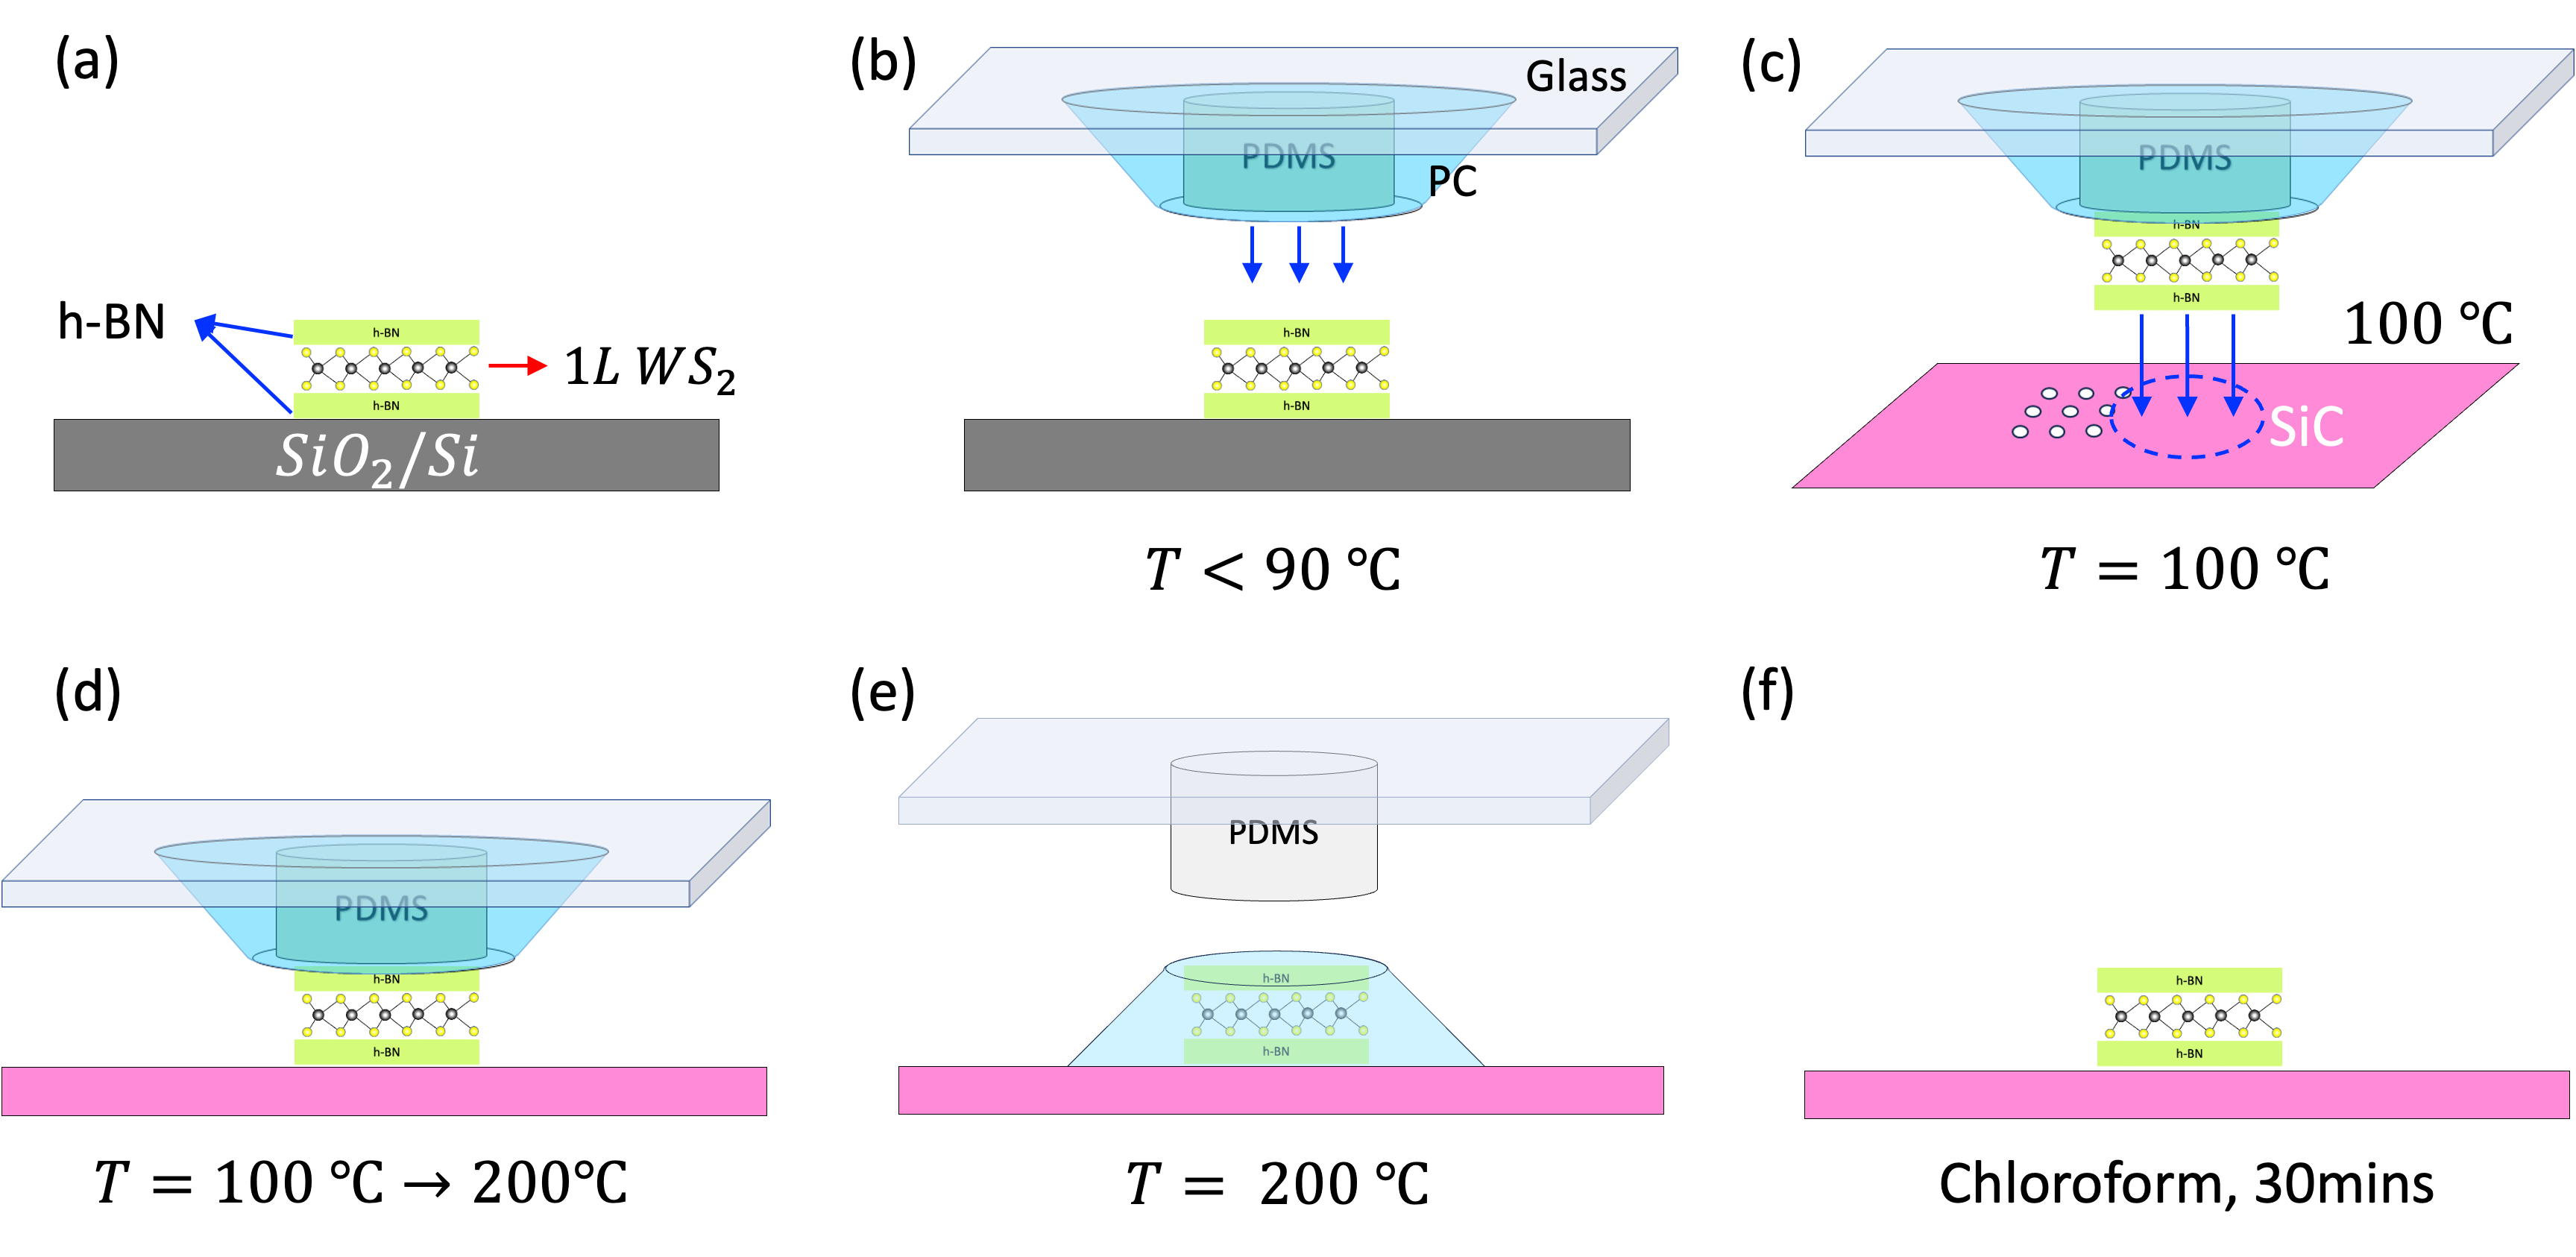
\includegraphics[width=\textwidth]{Figure/Chapter_methodology/PC_method.png}
	\caption{Hybrid PC-assisted transfer process. (a) Pre-assembly of an hBN-encapsulated monolayer $WS_2$ heterostructure on a sacrificial $SiO_2/Si$ substrate using PDMS-based dry transfer. (b) Pick-up of the heterostructure from the donor substrate using a PC stamp at $80^\circ$C. (c) Alignment of the PC-supported heterostructure with the target region on the suspended SiC membrane. (d) Thermal release process during heating from $100^\circ$C to $200^\circ$C. (e) Released heterostructure and sacrificial PC film on the SiC substrate after stamp retraction. (f) Final sample after removal of the PC film by immersion in chloroform for 30~min.}
	\label{fig:pc_method}
\end{figure}


The detailed procedure is illustrated in Fig.~\ref{fig:pc_method}. First, an hBN-encapsulated monolayer TMD stack is prepared on $SiO_2/Si$. The transfer stamp consists of a cylindrical PDMS support mounted on a glass slide and covered by a thin PC film. The PDMS support maintains a smooth and slightly curved PC surface. The PC stamp is then aligned with the pre-assembled heterostructure and brought into contact with the donor substrate. Mild heating to approximately $80^\circ$C increases the adhesion of the PC film, enabling the clean pick-up of the entire heterostructure.

After pick-up, the heterostructure supported by the PC film is aligned with the suspended SiC membrane. The stamp is lowered onto the target substrate while the stage temperature is increased from $100^\circ$C to $200^\circ$C. At this temperature, the PC softens sufficiently to release the stack onto the target area. Upon retraction of the glass slide, the sacrificial PC film and the heterostructure remain on the substrate, while the PDMS support remains attached to the slide. The final PC residue is then removed by immersing the sample in chloroform for 30~min, leaving a clean encapsulated heterostructure on the SiC membrane.



\begin{figure}[htbp]
	\centering
	\includegraphics[width=\textwidth]{Figure/Chapter_methodology/pickup.png}
	\caption{Optical microscopy images of the pick-up process for an hBN-encapsulated $WS_2$ monolayer using a PC/PDMS hybrid stamp. (a--c) The PC stamp is lowered and brought into contact with the heterostructure on the $SiO_2/Si$ donor substrate. (d--f) The hBN/$WS_2$ stack is picked up as the PC stamp is slowly retracted.}
	\label{fig:pickup}
\end{figure}


Fig.~\ref{fig:pickup} shows representative optical images recorded during the pick-up process. The hBN/$WS_2$ heterostructure is first prepared on a $SiO_2/Si$ donor substrate by PDMS-assisted transfer [Fig.~\ref{fig:pickup}(a)]. As the PC stamp approaches the surface, optical interference fringes appear, indicating the onset of contact between the PC film and the substrate [Fig.~\ref{fig:pickup}(b)]. With further lowering of the stamp, the contact area expands until it covers the entire heterostructure [Fig.~\ref{fig:pickup}(c)]. To promote efficient pick-up, the substrate is heated to $80^\circ$C, which increases the adhesion between the PC film and the heterostructure. The stamp is then slowly retracted. The final image [Fig.~\ref{fig:pickup}(f)] confirms that the heterostructure has been cleanly delaminated from the donor substrate and transferred onto the PC film.

\begin{figure}[htbp]
	\centering
	\includegraphics[width=\textwidth]{Figure/Chapter_methodology/transfer.png}
	\caption{Deterministic transfer of the hBN/$WS_2$ heterostructure onto a suspended SiC membrane. (a) Alignment of the stack on the PC stamp with the target membrane. (b,c) Initial contact and expansion of optical interference fringes as the stamp is lowered. (d) Full coverage of the heterostructure by the contact area. (e) Expansion of the contact area to the PC boundaries followed by thermal release at $200^\circ$C. (f) Final optical image after removal of the glass slide and PDMS support.}
	\label{fig:transfer}
\end{figure}

The subsequent transfer of the picked-up hBN/$WS_2$ heterostructure onto the SiC membrane is shown in Fig.~\ref{fig:transfer}. First, the stack supported by the PC film is aligned with the suspended membrane region [Fig.~\ref{fig:transfer}(a)]. As the stamp is lowered, the onset of contact is monitored through the appearance of optical interference fringes [Fig.~\ref{fig:transfer}(b)]. Further lowering causes the contact front to propagate outward, which helps to minimize trapped bubbles at the interface [Fig.~\ref{fig:transfer}(c)]. The process continues until the contact region fully covers the heterostructure and extends to the boundaries of the PC film [Fig.~\ref{fig:transfer}(d,e)]. The substrate is then heated to approximately $200^\circ$C to promote release of the PC film onto the target substrate. After retraction of the glass slide and PDMS support, the sacrificial PC layer and the embedded heterostructure remain on the chip. Fig.~\ref{fig:transfer}(f) shows the successfully transferred hBN/$WS_2$ heterostructure on the SiC membrane. This melt-release strategy enables reliable transfer of large-area flakes onto fragile suspended structures without introducing significant mechanical damage.

\subsection{Interface Optimization via Vacuum annealing} % (fold)


In nanomaterial fabrication, vacuum annealing is widely used to remove adsorbates, hydrocarbon residues, and other contaminants, thereby improving surface cleanliness and interface quality \cite{song-2019,han-2016,niesar-2010,park-2007}. For monolayer TMDs, this treatment is particularly important after exfoliation and transfer, since polymer residues and surface contamination can remain on the flakes and at buried interfaces \cite{haigh-2012,kretinin-2014}. Such contamination tends to accumulate into interfacial bubbles during stacking, leading to dielectric disorder, local doping, and inhomogeneous broadening of excitonic transitions. To reduce these effects, we introduced a vacuum-annealing step after each transfer process.

Annealing was carried out in a custom-built vacuum chamber [Fig.~\ref{fig:annealing}] equipped with a turbomolecular pump (Agilent TwisTorr 74 FS) backed by a dry scroll pump, yielding a base pressure below $10^{-7}$~Torr. The sample temperature was monitored using a PT100 temperature sensor in direct thermal contact with the heating stage. Its resistance was measured with a source-measure unit (Keithley 2400), and the temperature was determined from a calibrated resistance--temperature table (see Appendix). Following established protocols \cite{jain-2018,zhu-2017,kim-2018}, the samples were annealed at approximately $230^\circ$C for 30~min. This temperature is sufficiently high to remove transfer-related residues while remaining low enough to avoid structural degradation or unintended defect formation in the TMD monolayers. After annealing, the system was allowed to cool naturally to room temperature before the next fabrication step.

\begin{figure}[htbp]
	\centering
	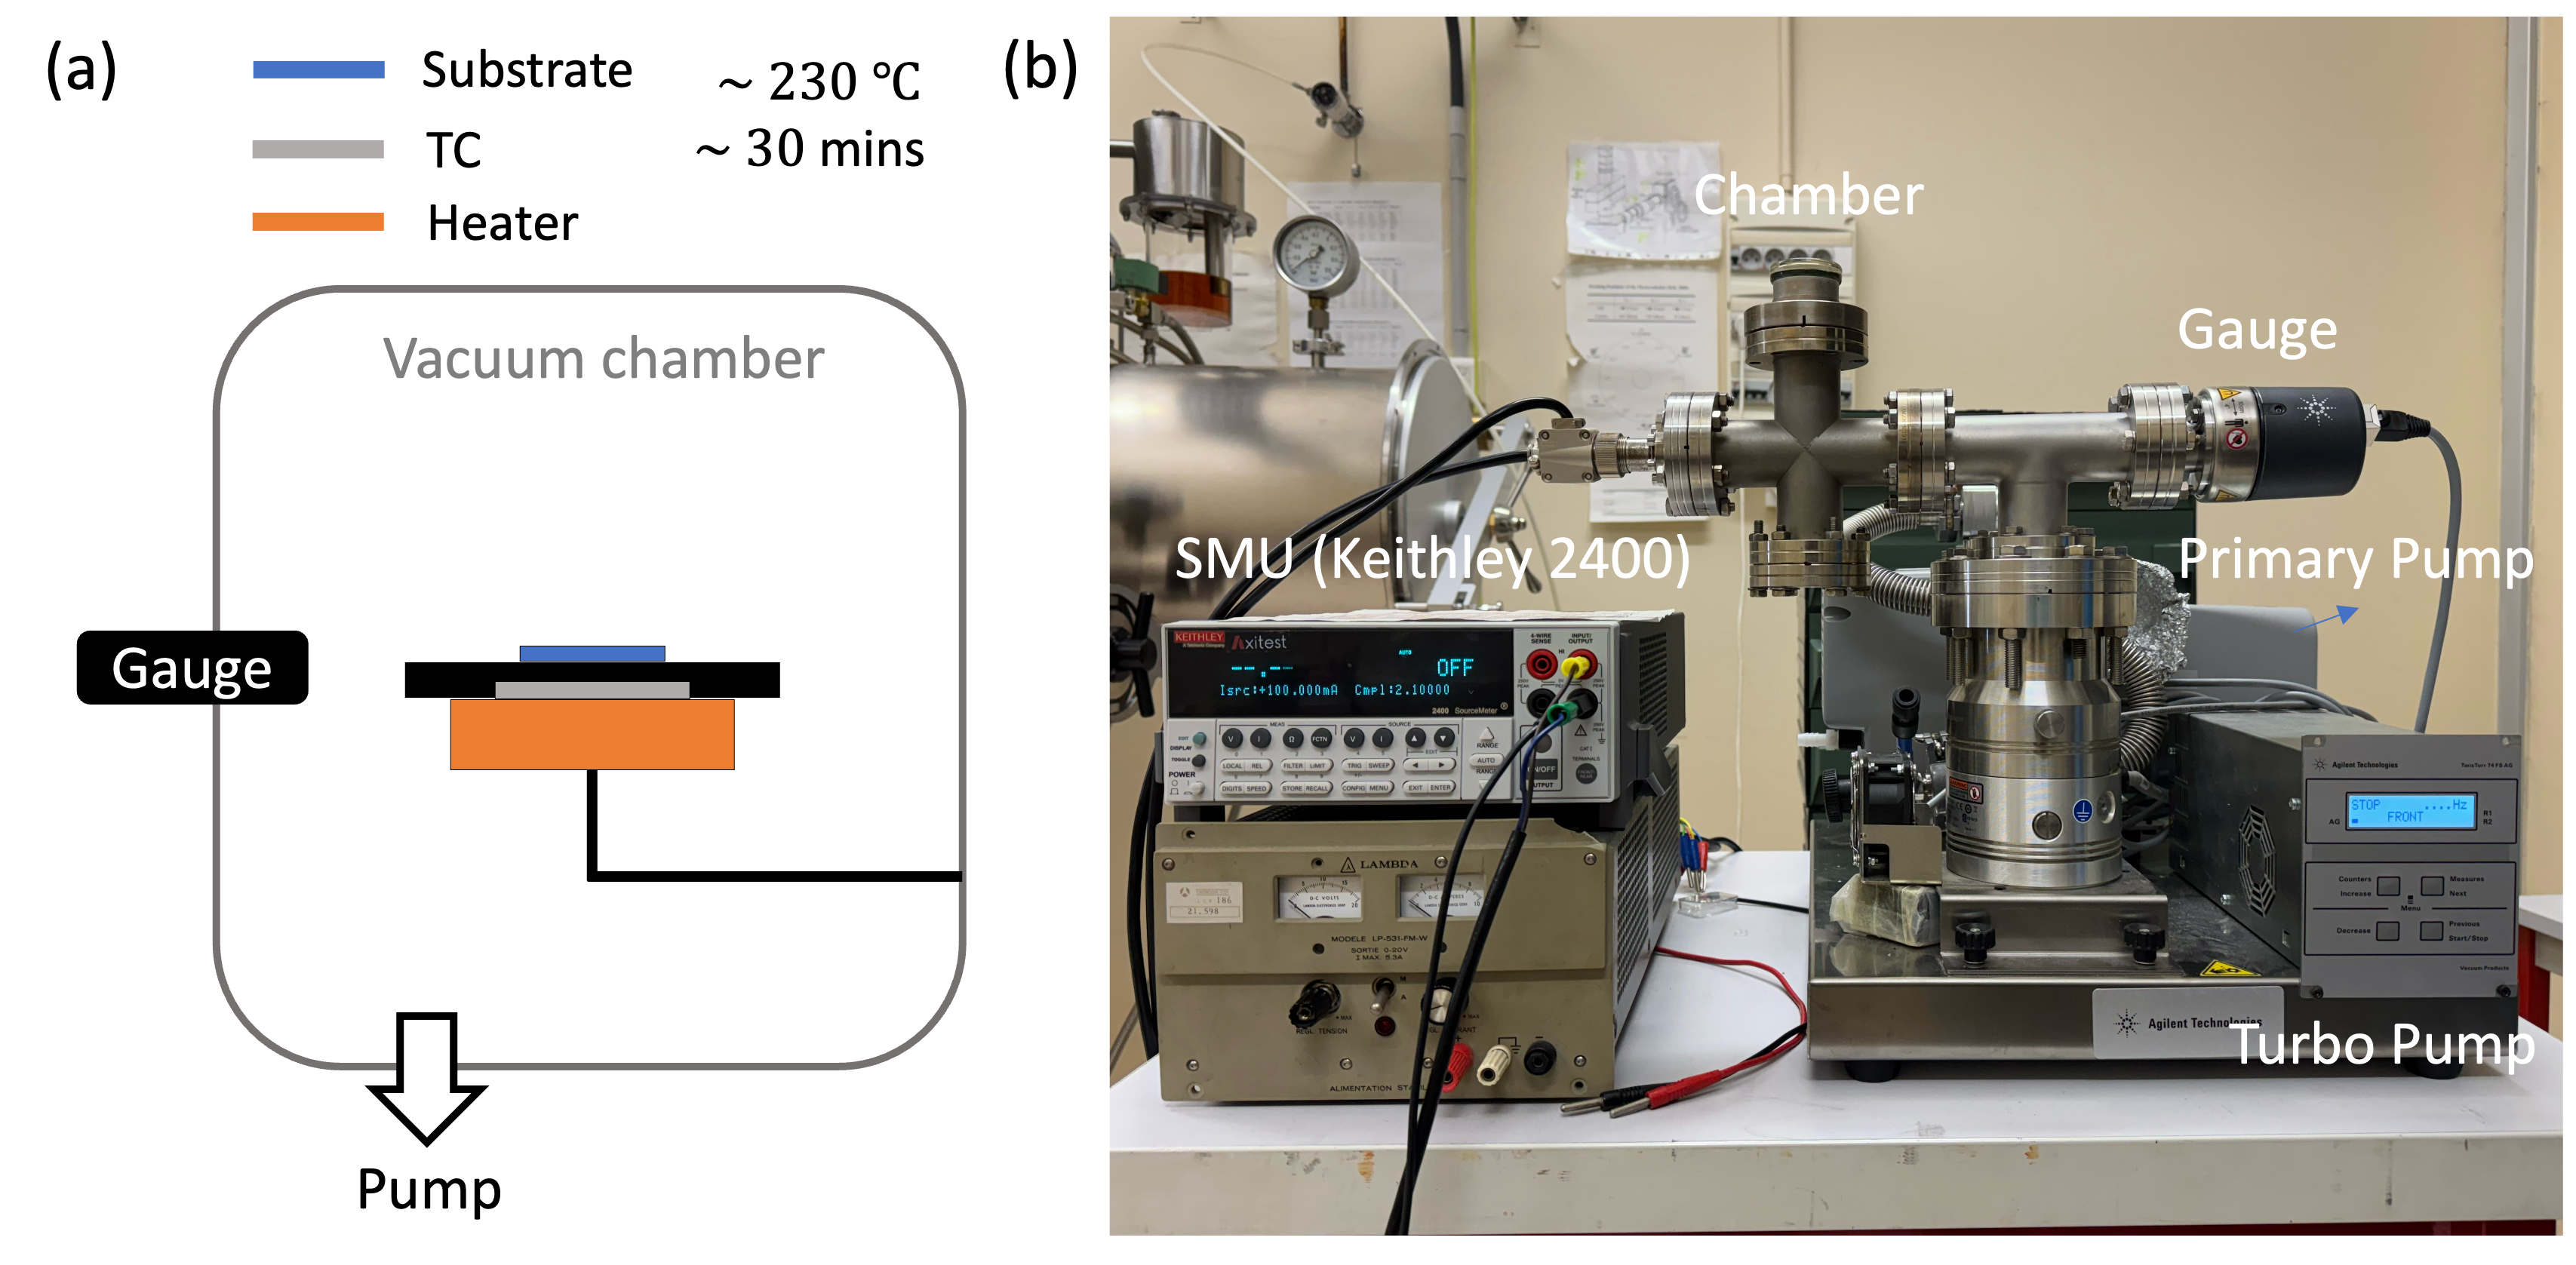
\includegraphics[width=\textwidth]{Figure/Chapter_methodology/annealing.png}
	\caption{(a) Schematic of the vacuum-annealing chamber. (b) Optical image of the annealing system.}
	\label{fig:annealing}
\end{figure}





\newpage



\section{Steady-state Optical Spectroscopy}
\label{sec:lipsum__section_3}

The experimental work presented in this thesis relies primarily on optical spectroscopy, with particular emphasis on photoluminescence (PL) measurements. As discussed in Chapter~1, the optical response of monolayer TMDs is dominated by excitonic effects. In the monolayer limit, the lack of inversion symmetry gives rise to two non-equivalent valleys at the $K^+$ and $K^-$ points of the Brillouin zone, each associated with distinct spin and valley selection rules \cite{xiao-2012,mak-2012}. These characteristics lead to a rich excitonic structure and make polarization-resolved spectroscopy a powerful probe of the underlying electronic states.

In monolayer $WS_2$, several excitonic complexes can only be clearly resolved at cryogenic temperatures. At room temperature ($\approx 300$~K), thermal broadening ($\approx 26$~meV) obscures many of the fine spectral features, often leaving only the neutral exciton and trion clearly visible \cite{plechinger-2016}, even in hBN-encapsulated samples \cite{mohamed-2017}. Low-temperature spectroscopy is therefore essential for resolving the underlying excitonic structure \cite{zinkiewicz-2021c}. In addition, polarization-resolved excitation and detection are required to access the intrinsic spin-valley coupling of these materials. For this reason, our optical platform combines cryogenic operation with high-precision polarization control.



\subsection{Optical Setup (Polarization-resolved)}
\label{subsec:optical_setup}

To investigate the optical properties of monolayer TMDs, we developed a polarization-resolved micro-spectroscopy system that combines cryogenic excitation with high-sensitivity photoluminescence detection. A schematic of the setup is shown in Fig.~\ref{fig:optical_setup}. The overall configuration combines excitation, polarization control, and detection in a single optical path, enabling both steady-state and time-resolved measurements within the same platform.

\begin{figure}[htbp]
    \centering
    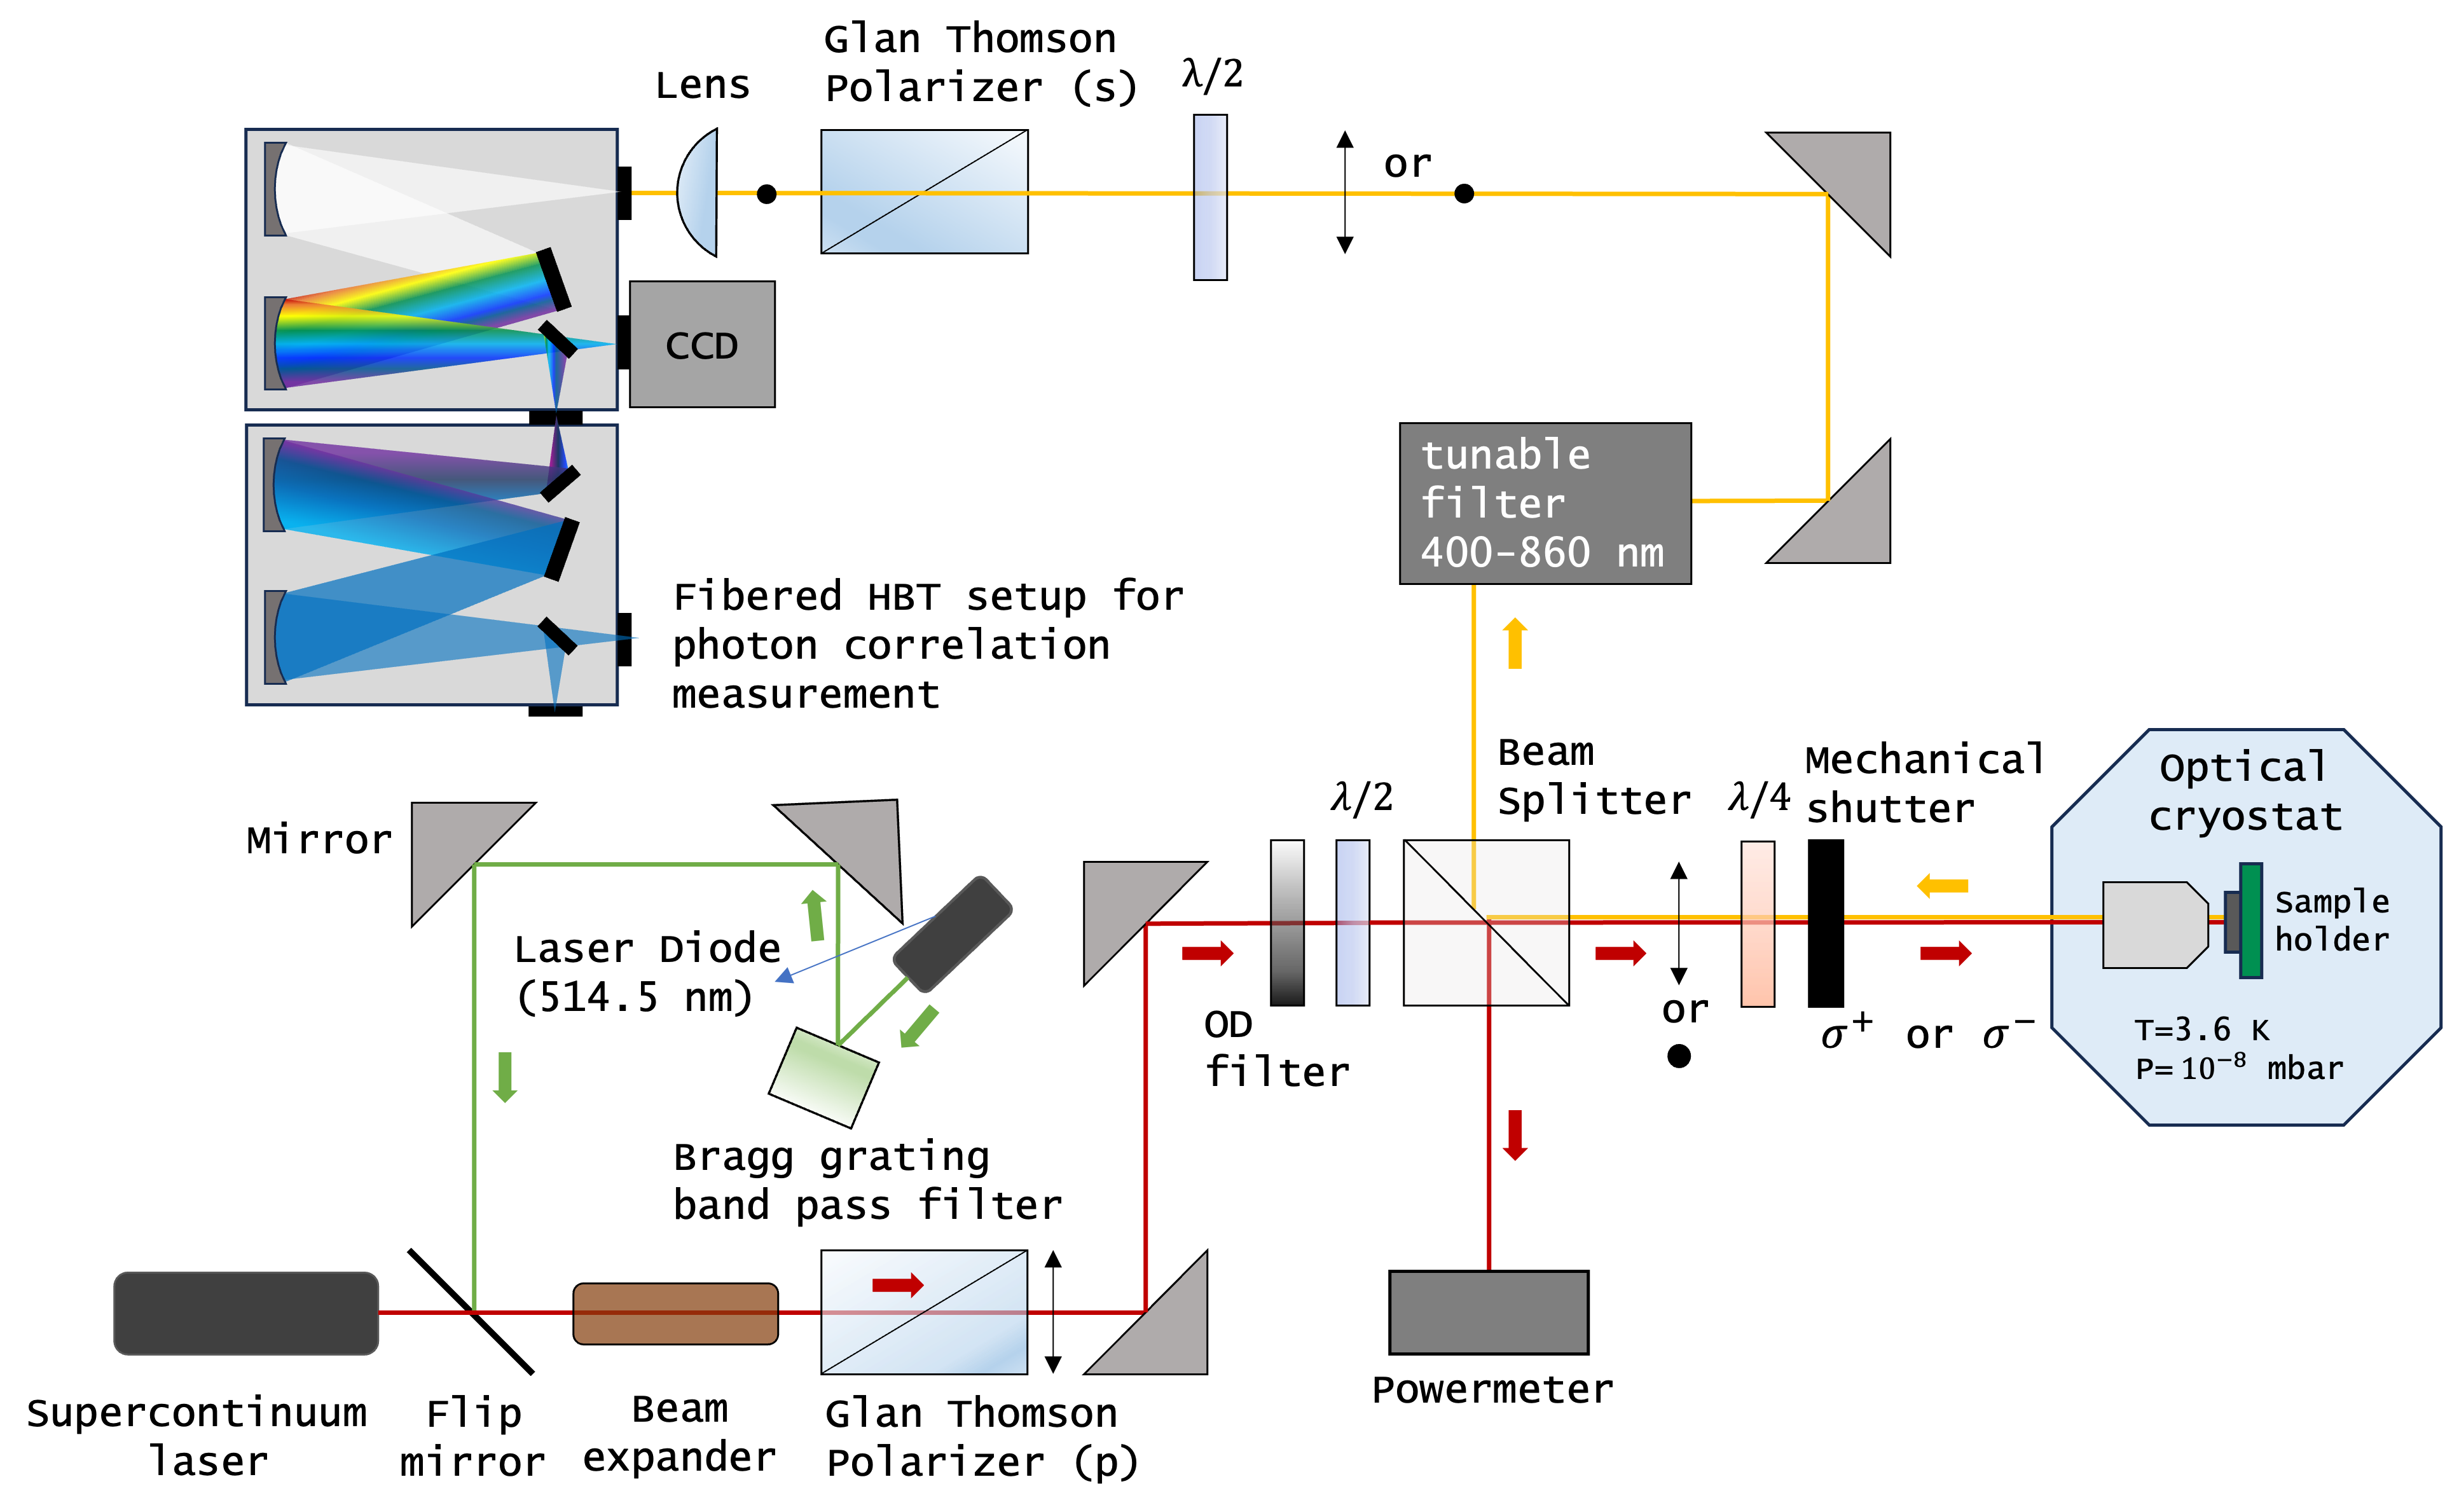
\includegraphics[width=0.9\textwidth]{Figure/Chapter_methodology/optical_setup.png}
    \caption{Optical setup for $\mu$-photoluminescence spectroscopy.}
    \label{fig:optical_setup}
\end{figure}

\vspace{1em}
\noindent \textbf{Excitation sources and beam conditioning} \\

The setup incorporates two excitation sources that can be selected using a flip mirror, depending on the measurement mode. The primary source is a pulsed supercontinuum laser (NKT SuperK), which provides a tunable spectral range from 400 to 1100~nm. Owing to its broad tunability and pulsed operation, it is used for most measurements, including photoluminescence (PL), photoluminescence excitation (PLE), and time-resolved photoluminescence (TRPL). In addition, a 514.5~nm continuous-wave laser diode equipped with a Bragg-grating bandpass filter is available for steady-state measurements requiring fixed-wavelength excitation.

The selected beam is expanded and collimated so as to overfill the back aperture of the objective lens, thereby maximizing the effective numerical aperture and enabling diffraction-limited focusing. According to the Rayleigh criterion, the lateral spatial resolution $d$ is given by
\begin{equation}
d = 1.22 \frac{\lambda}{NA}.
\end{equation}
This configuration provides a sub-micrometer excitation spot, allowing spatially selective measurements on individual flakes and localized emission centers.




\vspace{1em}
\noindent \textbf{Excitation path} \\

To probe valley-selective excitonic responses, the excitation path is designed to precisely control the helicity of the incident light. The beam first passes through a Glan--Thompson polarizer to define a high-purity linear polarization state. A half-wave plate (HWP) is then used to adjust the polarization orientation. After passing through a beam splitter, an optical-density filter, and a mechanical shutter, the beam is converted into either right- ($\sigma^+$) or left- ($\sigma^-$) circularly polarized light using a quarter-wave plate (QWP). This configuration enables selective excitation of the $K^+$ and $K^-$ valleys in the monolayer.

\vspace{1em}
\noindent \textbf{Emission path} \\

The photoluminescence emitted by the sample is collected by the same objective and directed into the detection path. The circular polarization components are converted back into orthogonal linear polarizations by the QWP. After reflection by the beam splitter and spectral filtering, polarization analysis is performed using a second HWP and a fixed Glan--Thompson polarizer. By rotating the HWP, each polarization component can be selectively projected onto the detection axis prior to spectral or temporal analysis.



% [Image of a polarization analyzer setup using a half-wave plate and a polarizer]


\vspace{1em}
\noindent \textbf{Signal detection and spectral analysis} \\

After polarization selection, the signal is coupled into a double-spectrometer system to ensure high spectral purity and efficient suppression of stray light. The first spectrometer, equipped with a thermoelectrically cooled CCD camera (PIXIS 100, Princeton Instruments), is used for high-resolution spectral measurements and PL mapping. Alternatively, the signal can be directed to a second spectrometer acting as a tunable narrow bandpass filter. By adjusting its central wavelength and exit slit width, individual emission lines can be spectrally isolated for time-resolved and photon-correlation measurements.

The filtered signal is then coupled into a fiber-based detection system. For TRPL measurements, the emission is sent to a single-photon avalanche diode (SPAD), and the photon arrival times are recorded relative to the laser synchronization signal. For photon-correlation measurements, a Hanbury Brown--Twiss interferometer is implemented using a 50:50 multimode fiber coupler (50~$\mu$m core, Thorlabs) and two SPADs. The electronic signals are processed by a time-correlated single-photon counting module (PicoHarp 300, PicoQuant), enabling the measurement of excitonic lifetimes and the reconstruction of the second-order coherence function, $g^{(2)}(\tau)$.


\subsection{Polarization-resolved Photoluminescence (PL) Measurements}
\label{subsec:polarization_pl}


Photoluminescence (PL) refers to the emission of photons following optical excitation. When a semiconductor is illuminated with photons of energy exceeding its bandgap ($h\nu > E_g$), electrons are promoted to the conduction band, leaving holes in the valence band. In monolayer TMDs, strong Coulomb interactions lead to the formation of tightly bound excitons. After excitation, carriers relax toward lower-energy states and recombine radiatively, giving rise to photon emission.

% \begin{enumerate}
%     \item \textbf{Excitation}: absorption of an incident photon generates an electron--hole pair.
%     \item \textbf{Relaxation}: carriers excited far above the band edge lose energy through scattering and phonon-assisted relaxation toward lower-energy states.
%     \item \textbf{Recombination}: radiative recombination of the electron and hole gives rise to photon emission.
% \end{enumerate}

In monolayer TMDs, the exciton binding energy is unusually large, typically in the range of 0.3--0.7~eV \cite{chernikov-2014}, owing to reduced dielectric screening and quantum confinement in the two-dimensional limit. As a result, excitons remain stable even at room temperature, making these materials particularly well suited for studies of excitonic and valley-dependent optical phenomena.


\begin{figure}[htbp]
    \centering
    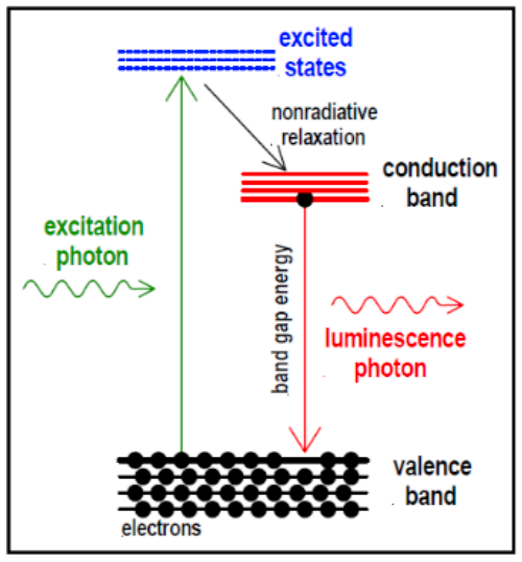
\includegraphics[width=0.5\textwidth]{Figure/Chapter_methodology/pl_process.png}
    \caption{Principle of photoluminescence spectroscopy (PL) \cite{vuong-2018}.}
    \label{fig:pl_mechanism}
\end{figure}

Although conventional PL spectroscopy provides information on emission energies and intensities, it does not distinguish between contributions from the two inequivalent valleys. To probe valley-dependent optical selection rules and circular dichroism in monolayer TMDs \cite{xiao-2012,cao-2012,mak-2012}, polarization-resolved PL measurements are required. By controlling the helicity of both excitation and detection, one can selectively initialize and analyze valley-polarized excitonic populations.

\begin{figure}[htbp]
    \centering
    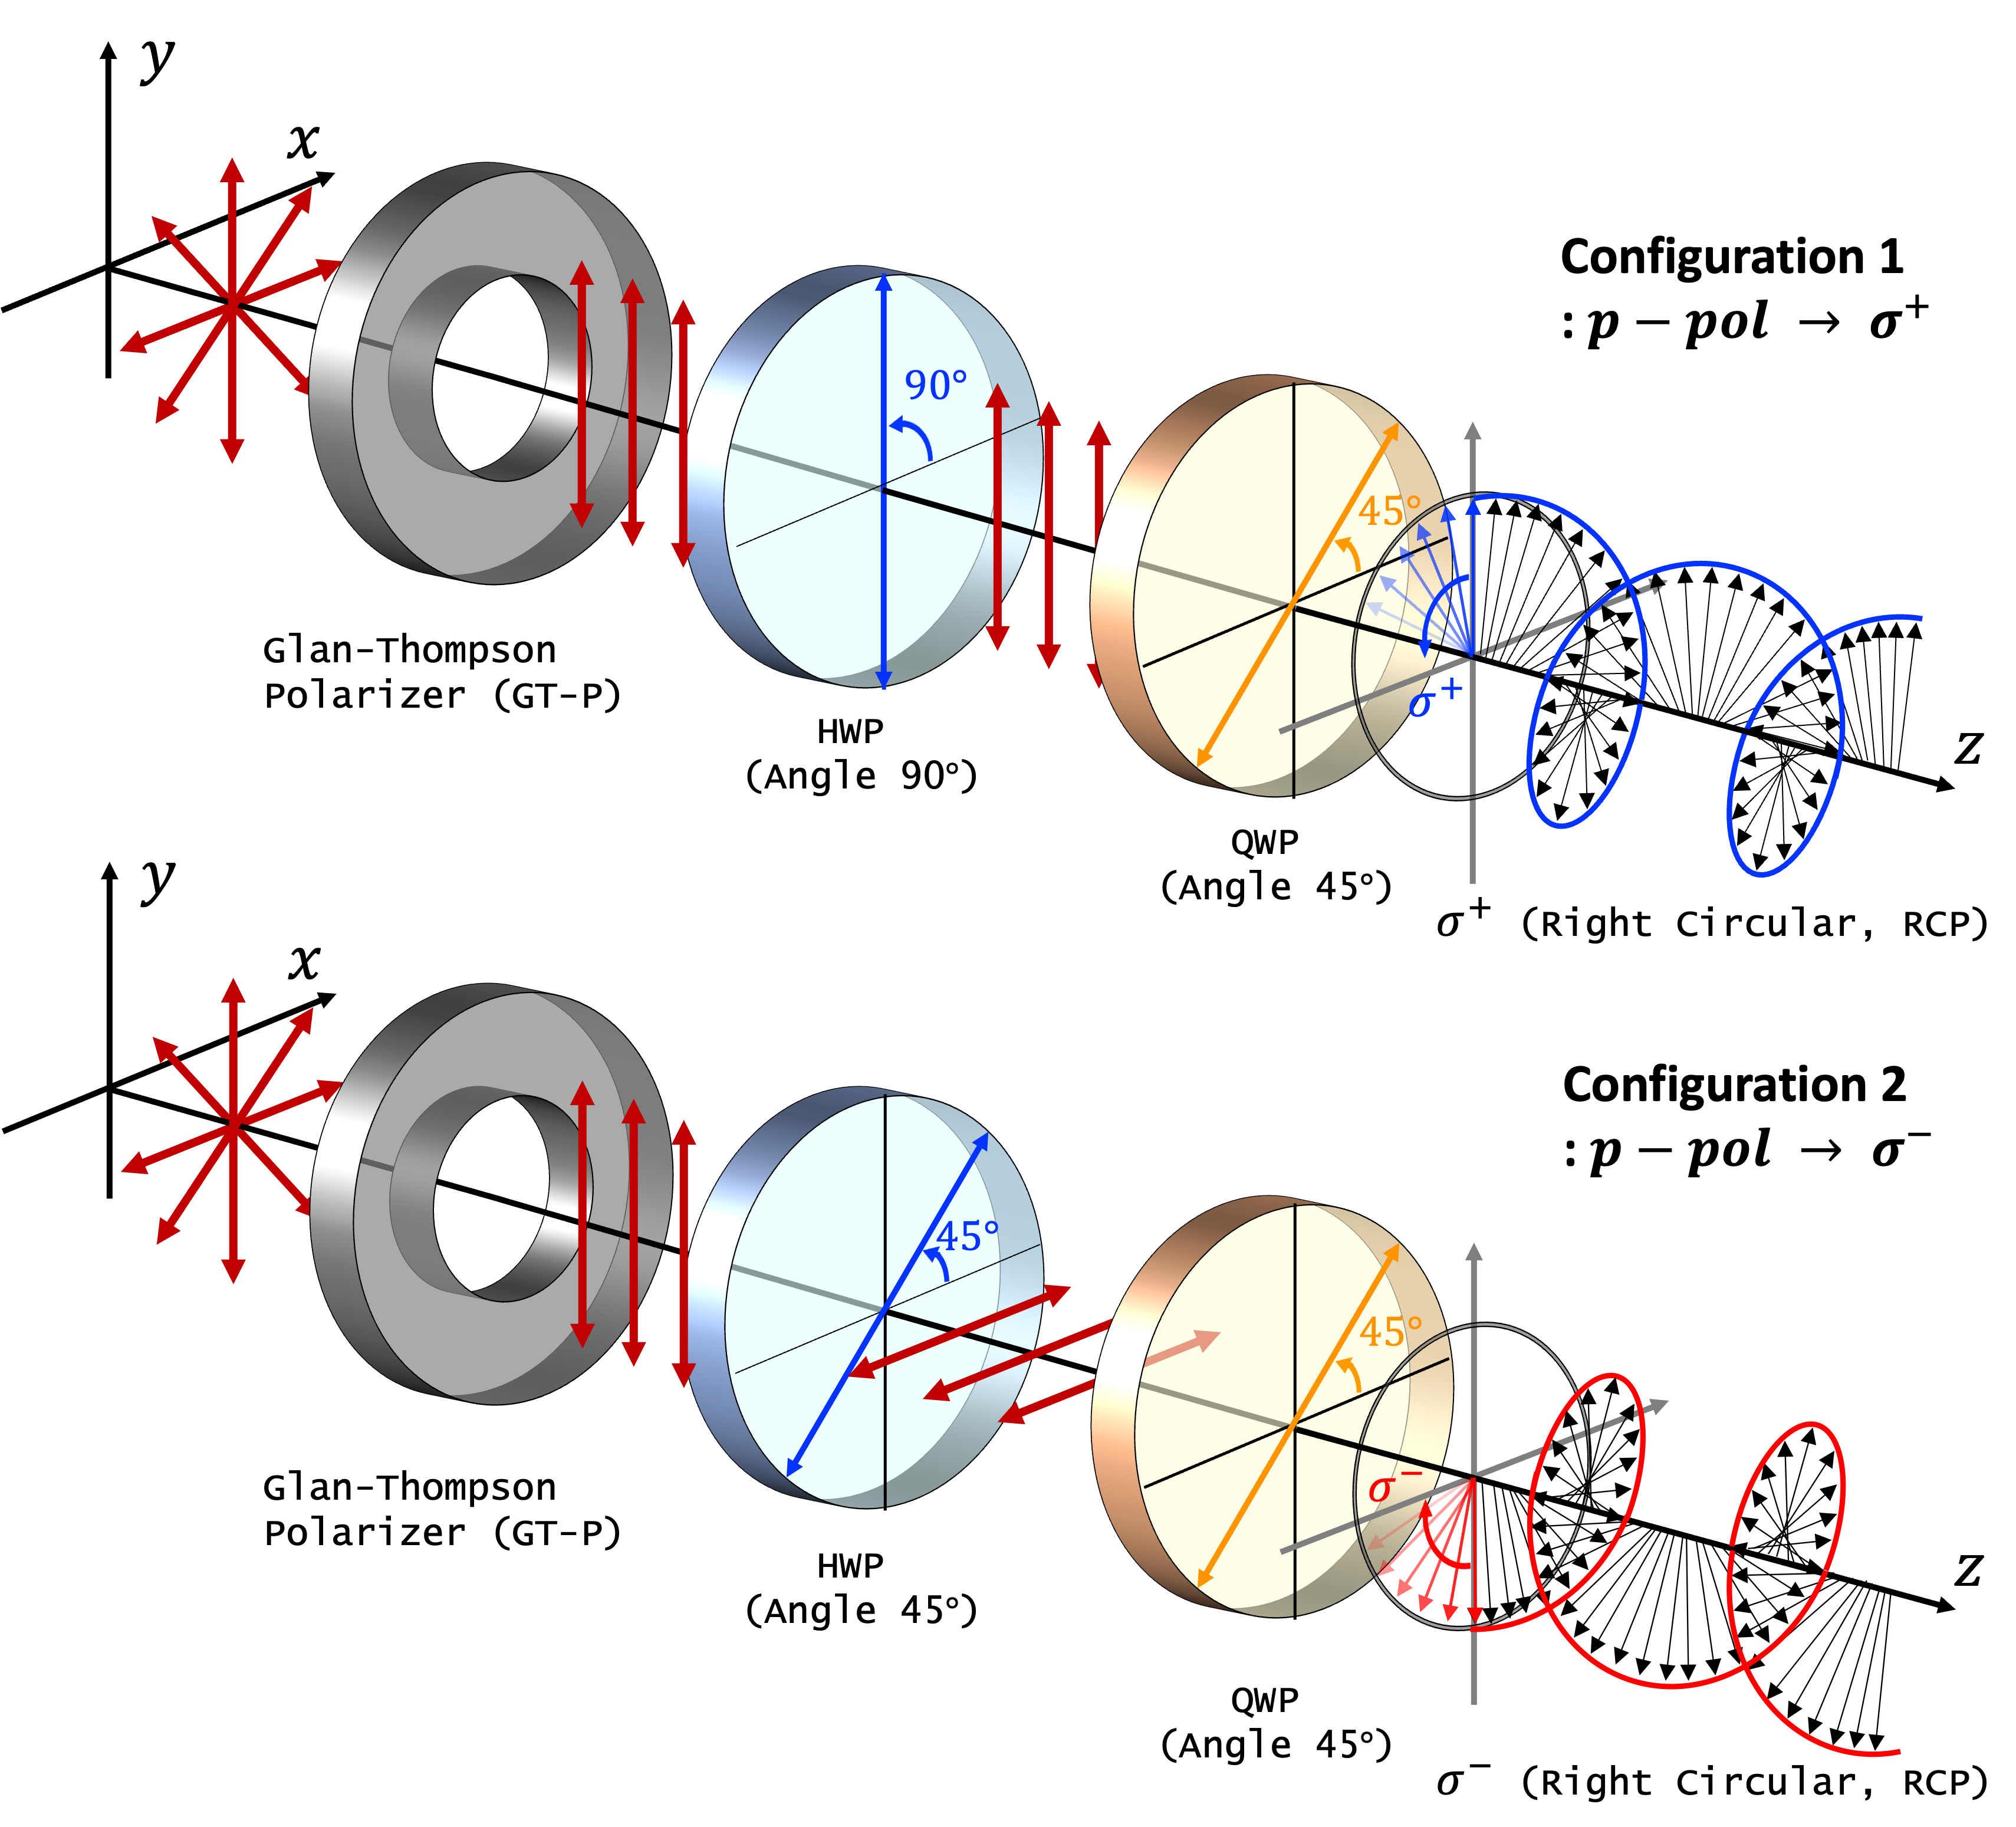
\includegraphics[width=0.9\textwidth]{Figure/Chapter_methodology/polarization.png}
	\caption{Schematic diagram of the generation and analysis of circularly polarized light.}
    \label{fig:polarization_setup}
\end{figure}

Fig.~\ref{fig:polarization_setup} illustrates the optical generation of circularly polarized light. The excitation beam is first linearly polarized using a Glan--Thompson polarizer and then passed through a half-wave plate (HWP), which controls the polarization orientation. A subsequent quarter-wave plate (QWP), oriented at $45^\circ$, converts the linear polarization into either right- ($\sigma^+$) or left- ($\sigma^-$) circularly polarized light, depending on the HWP angle.

Upon emission, the circularly polarized components are converted back into orthogonal linear polarizations by the same QWP. The selection of the emission helicity is achieved using a second HWP placed before a fixed linear polarizer. By rotating this HWP, either the $\sigma^+$ or $\sigma^-$ component can be projected onto the detection axis, enabling sequential acquisition of the polarization-resolved spectra. This configuration ensures high stability and reproducibility in the polarization analysis.

A more rigorous description of the polarization transformations can be obtained using Jones calculus, which is presented in Appendix~X.

The polarization properties of the emission are quantified using the degree of circular polarization (DOCP) and the degree of linear polarization (DOLP), defined as:
\begin{equation}
    \text{DOCP} = \frac{I_{\sigma^+\sigma^+} - I_{\sigma^+\sigma^-}}{I_{\sigma^+\sigma^+} + I_{\sigma^+\sigma^-}}, \quad
    \text{DOLP} = \frac{I_{\pi\pi} - I_{\pi\bar{\pi}}}{I_{\pi\pi} + I_{\pi\bar{\pi}}}
\end{equation}
where $I_{\sigma^+\sigma^+}$ ($I_{\pi\pi}$) and $I_{\sigma^+\sigma^-}$ ($I_{\pi\bar{\pi}}$) denote the co-polarized and cross-polarized intensities, respectively. A finite DOCP reflects a population imbalance between the two valleys, while a non-zero DOLP indicates coherent superposition between valley states.

For improved robustness against experimental asymmetries, the DOCP can be determined using a double-ratio method \cite{sato-1981}:
\begin{equation}
    \text{DOCP} = \frac{\sqrt{I_{++} I_{--}} - \sqrt{I_{+-} I_{-+}}}{\sqrt{I_{++} I_{--}} + \sqrt{I_{+-} I_{-+}}} \times 100\%
\end{equation}

This approach reduces the influence of fluctuations in excitation power and detection efficiency. Furthermore, access to both circular and linear polarization bases allows the evaluation of the ratio between total circular and linear emission intensities ($I_{\sigma}/I_{\pi}$). This ratio provides insight into the interplay between valley population and quantum coherence, where $I_{\sigma}$ reflects the population imbalance between valleys, while $I_{\pi}$ probes their coherent superposition.

% Figure \ref{fig:polarization_setup} illustrates the optical transition from $p$-polarized light to either right ($\sigma^+$) or left ($\sigma^-$) circularly polarized light. Initially, the light is aligned in the vertical direction ($p$-pol) by passing through a Glan-Thompson polarizer ($\text{GTP}_p$) and is then directed to a half-wave plate (HWP). In \textbf{Configuration 1}, the fast axis of the HWP is aligned vertically ($90^\circ$ relative to the $x$-axis). Since the $p$-polarized light is parallel to the fast axis, it passes through the HWP without any change in polarization. This light then encounters a quarter-wave plate (QWP) oriented at $45^\circ$. Because the polarization of the light is at a $+45^\circ$ angle relative to the fast axis of the QWP, it is converted into right circularly polarized light ($\sigma^+$).

% In contrast, in \textbf{Configuration 2}, the HWP is rotated to $45^\circ$. The incident $p$-polarized light meets the HWP at a $45^\circ$ angle, which rotates the polarization to the horizontal direction ($s$-pol). As this $s$-polarized light reaches the QWP, it has an angle of $-45^\circ$ relative to the QWP's fast axis, resulting in the production of left circularly polarized light ($\sigma^-$). Consequently, both $\sigma^+$ and $\sigma^-$ light can be produced simply by changing the angle of the HWP.

% Following the emission from the sample, the combination of right- ($\sigma^+$) and left- ($\sigma^-$) circularly polarized light is transformed back into a combination of $p$-polarized and $s$-polarized linear light after passing through the QWP. To selectively measure each component using a spectrometer, a second Glan-Thompson polarizer ($\text{GTP}_s$), fixed to the $s$-polarization axis, is placed at the end of the optical path. 

% The selection of the specific helicity is controlled by an additional HWP placed immediately before the $\text{GTP}_s$. If the HWP is set to its neutral axis ($\theta_H = 90^\circ$), the linear combination of $p$-pol and $s$-pol light experiences no change in polarization; thus, only the $s$-polarized component (originally $\sigma^-$) passes through the $\text{GTP}_s$ to the spectrometer. Conversely, to measure the $\sigma^+$ component, the HWP is rotated to $45^\circ$, which effectively switches the polarizations: the $p$-pol component (originally $\sigma^+$) is converted to $s$-pol, while the original $s$-pol is converted to $p$-pol. This allows the signal corresponding to $\sigma^+$ to pass through the $\text{GTP}_s$. In summary, we can sequentially extract the spectra for both $\sigma^+$ and $\sigma^-$ by simply toggling the HWP between $45^\circ$ and its neutral position, ensuring high mechanical stability and alignment consistency during the measurement.

% To provide a more rigorous description of the polarization states, we employ the complex analytic representation and the Jones calculus framework. Following the physics convention ($kz - \omega t$), the electric field of the incident light—initially linearly polarized in the vertical direction ($p$-pol) by a $\text{GTP}_p$ and propagating in the $+z$ direction—can be mathematically expressed as:
% \begin{equation}
% \mathbf{E}_p(z, t) = E_0 e^{i(kz - \omega t)} \hat{\mathbf{y}} = E_0 e^{i(kz - \omega t)} \begin{pmatrix} 0 \\ 1 \end{pmatrix}
% \end{equation}

% By extracting the complex amplitude vector from this representation, we can define the polarization state within the Jones calculus framework as the Jones vector $\mathbf{J}_{in}$:
% \begin{equation}
% \mathbf{J}_{in} = \begin{pmatrix} 0 \\ 1 \end{pmatrix}
% \end{equation}

% The transformation of the incident light is first controlled by a half-wave plate (HWP). The general Jones matrix for a HWP with its fast axis at an angle $\theta_H$ is defined as:
% \begin{equation}
%     M_{HWP}(\theta_H) = \begin{pmatrix} \cos 2\theta_H & \sin 2\theta_H \\ \sin 2\theta_H & -\cos 2\theta_H \end{pmatrix}
% \end{equation}

% For the two primary experimental configurations, the HWP converts the incident $p$-polarized light into either $p$- or $s$-polarized states as follows:
% \begin{itemize}
%     \item \textbf{Configuration 1} ($\theta_H = 90^\circ$):
%     \begin{equation}
%         \mathbf{J}_{HWP} = M_{HWP}(90^\circ) \begin{pmatrix} 0 \\ 1 \end{pmatrix} = \begin{pmatrix} -1 & 0 \\ 0 & 1 \end{pmatrix} \begin{pmatrix} 0 \\ 1 \end{pmatrix} = \begin{pmatrix} 0 \\ 1 \end{pmatrix}
%     \end{equation}
%     \item \textbf{Configuration 2} ($\theta_H = 45^\circ$):
%     \begin{equation}
%         \mathbf{J}_{HWP} = M_{HWP}(45^\circ) \begin{pmatrix} 0 \\ 1 \end{pmatrix} = \begin{pmatrix} 0 & 1 \\ 1 & 0 \end{pmatrix} \begin{pmatrix} 0 \\ 1 \end{pmatrix} = \begin{pmatrix} 1 \\ 0 \end{pmatrix}
%     \end{equation}
% \end{itemize}

% These states are then passed through a quarter-wave plate (QWP) fixed at $\theta_Q = 45^\circ$. The general Jones matrix for a QWP is given by:
% \begin{equation}
% M_{QWP}(\theta_Q) = \begin{pmatrix} \cos^2 \theta_Q + i \sin^2 \theta_Q & (1-i) \sin \theta_Q \cos \theta_Q \\ (1-i) \sin \theta_Q \cos \theta_Q & \sin^2 \theta_Q + i \cos^2 \theta_Q \end{pmatrix}
% \end{equation}
% Substituting $\theta_Q = 45^\circ$ yields $M_{QWP}(45^\circ) = \frac{1}{2} \begin{pmatrix} 1+i & 1-i \\ 1-i & 1+i \end{pmatrix}$, resulting in the output Jones vectors for each configuration:
% \begin{itemize}
%     \item \textbf{Configuration 1}: $\mathbf{J}_{out} = M_{QWP}(45^\circ) \begin{pmatrix} 0 \\ 1 \end{pmatrix} = \frac{1}{2} \begin{pmatrix} 1-i \\ 1+i \end{pmatrix} \equiv \frac{1}{\sqrt{2}} \begin{pmatrix} 1 \\ i \end{pmatrix} = \mathbf{J}_{\sigma^+}$
%     \item \textbf{Configuration 2}: $\mathbf{J}_{out} = M_{QWP}(45^\circ) \begin{pmatrix} 1 \\ 0 \end{pmatrix} = \frac{1}{2} \begin{pmatrix} 1+i \\ 1-i \end{pmatrix} \equiv \frac{1}{\sqrt{2}} \begin{pmatrix} 1 \\ -i \end{pmatrix} = \mathbf{J}_{\sigma^-}$
% \end{itemize}

% Upon excitation, the emitted light can be described as a linear combination of circular components: $\mathbf{E}_{em} = a_+ \mathbf{J}_{\sigma^+} + a_- \mathbf{J}_{\sigma^-}$. The light propagates back through the same QWP. To maintain a consistent mathematical description for this reverse propagation, we redefine the coordinate system ($x' = -x$). In this redefined frame, the QWP's fast axis is oriented at $135^\circ$ relative to the new $x'$-axis:
% \begin{equation}
%     M_{QWP}(135^\circ) = \frac{1}{2} \begin{pmatrix} 1+i & -1+i \\ -1+i & 1+i \end{pmatrix}
% \end{equation}

% The final polarization state $\mathbf{J}_{det}$ after the QWP maps each circular component onto orthogonal linear states as follows:
% \begin{itemize}
%     \item \textbf{For the $\sigma^+$ component:}
%     \begin{equation}
%     \begin{aligned}
%         M_{QWP}(135^\circ) \mathbf{J}_{\sigma^+} &= \frac{1}{2\sqrt{2}} \begin{pmatrix} 1+i & -1+i \\ -1+i & 1+i \end{pmatrix} \begin{pmatrix} 1 \\ i \end{pmatrix} \\
%         &= \frac{1}{2\sqrt{2}} \begin{pmatrix} (1+i) + (-1+i)i \\ (-1+i) + (1+i)i \end{pmatrix} \\
%         &= \frac{1}{2\sqrt{2}} \begin{pmatrix} 1+i-i+i^2 \\ -1+i+i+i^2 \end{pmatrix} = \frac{-1+i}{\sqrt{2}} \begin{pmatrix} 0 \\ 1 \end{pmatrix} \propto \mathbf{J}_V
%     \end{aligned}
%     \end{equation}
%     \item \textbf{For the $\sigma^-$ component:}
%     \begin{equation}
%     \begin{aligned}
%         M_{QWP}(135^\circ) \mathbf{J}_{\sigma^-} &= \frac{1}{2\sqrt{2}} \begin{pmatrix} 1+i & -1+i \\ -1+i & 1+i \end{pmatrix} \begin{pmatrix} 1 \\ -i \end{pmatrix} \\
%         &= \frac{1}{2\sqrt{2}} \begin{pmatrix} (1+i) - (-1+i)i \\ (-1+i) - (1+i)i \end{pmatrix} \\
%         &= \frac{1}{2\sqrt{2}} \begin{pmatrix} 1+i+i-i^2 \\ -1+i-i-i^2 \end{pmatrix} = \frac{1+i}{\sqrt{2}} \begin{pmatrix} 1 \\ 0 \end{pmatrix} \propto \mathbf{J}_H
%     \end{aligned}
%     \end{equation}
% \end{itemize}

% The final Jones vector reaching the detector is determined by the configuration of the second HWP placed before the fixed $\text{GTP}_s$ (oriented to the $s$-polarization axis). The HWP acts on the mapped linear states, $\mathbf{J}_{det} \propto a_+ \mathbf{J}_V + a_- \mathbf{J}_H$, as follows:

% \begin{itemize}
%     \item \textbf{Neutral Axis ($\theta_H = 90^\circ$):} 
%     The HWP matrix $M_{HWP}(90^\circ)$ leaves the orthogonal states essentially unchanged in their linear orientation:
%     \begin{equation}
%         M_{HWP}(90^\circ) (a_+ \mathbf{J}_V + a_- \mathbf{J}_H) = \begin{pmatrix} -1 & 0 \\ 0 & 1 \end{pmatrix} \left[ a_+ \begin{pmatrix} 0 \\ 1 \end{pmatrix} + a_- \begin{pmatrix} 1 \\ 0 \end{pmatrix} \right] = \begin{pmatrix} -a_- \\ a_+ \end{pmatrix}
%     \end{equation}
%     In this configuration, the $V$-polarized component ($a_+$) is blocked by the $\text{GTP}_s$, while the $H$-polarized component (originally $\sigma^-$) passes through to be detected.

%     \item \textbf{Switching Axis ($\theta_H = 45^\circ$):} 
%     The HWP matrix $M_{HWP}(45^\circ)$ swaps the $p$- and $s$-polarization components:
%     \begin{equation}
%         M_{HWP}(45^\circ) (a_+ \mathbf{J}_V + a_- \mathbf{J}_H) = \begin{pmatrix} 0 & 1 \\ 1 & 0 \end{pmatrix} \left[ a_+ \begin{pmatrix} 0 \\ 1 \end{pmatrix} + a_- \begin{pmatrix} 1 \\ 0 \end{pmatrix} \right] = \begin{pmatrix} a_+ \\ a_- \end{pmatrix}
%     \end{equation}
%     By rotating the HWP to $45^\circ$, the original $\sigma^+$ component ($a_+$) is converted into $H$-polarization, allowing it to pass through the $\text{GTP}_s$ for measurement.
% \end{itemize}

% Consequently, the measured intensity $I \propto |\mathbf{J}_{det}|^2$ selectively yields the spectra of $a_-$ and $a_+$ for $\theta_H = 90^\circ$ and $45^\circ$, respectively, providing a robust and precise determination of the valley-polarized photoluminescence.

% Beyond the circular polarization configuration, this optical setup also provides a straightforward means to characterize linear polarization states. By aligning the fast axis of the quarter-wave plate (QWP) with its neutral axis, the QWP no longer induces a phase delay between the orthogonal components, effectively acting as a transparent window for the incident linear states. This versatility allows for a comprehensive investigation of both the valley-dependent circular dichroism and the underlying linear polarization anisotropy within the same experimental framework.


% Leveraging the versatility of this polarization control system, we can seamlessly characterize both circular ($\sigma$) and linear ($\pi$) polarization states within a unified experimental framework. Initially, the polarization purity can be evaluated using simplified two-component measurements under a fixed excitation condition. For instance, the \textbf{Degree of Circular Polarization (DOCP)} and the \textbf{Degree of Linear Polarization (DOLP)} are extracted as follows:
% \begin{equation}
%     \text{DOCP} = \frac{I_{\sigma^+\sigma^+} - I_{\sigma^+\sigma^-}}{I_{\sigma^+\sigma^+} + I_{\sigma^+\sigma^-}}, \quad \text{DOLP} = \frac{I_{\pi\pi} - I_{\pi\bar{\pi}}}{I_{\pi\pi} + I_{\pi\bar{\pi}}}
% \end{equation}
% where $I_{\sigma^+\sigma^+}$ ($I_{\pi\pi}$) and $I_{\sigma^+\sigma^-}$ ($I_{\pi\bar{\pi}}$) represent the co-polarized and cross-polarized intensities for each basis, respectively.

% Generally, however, utilizing all four combinations ($\sigma_{++}, \sigma_{+-}, \sigma_{--}, \sigma_{-+}$) provides a significant advantage in suppressing any spurious effects due to the optics’ eventual birefringence or polarization-dependent response. By incorporating the full set of measurements, the DOCP is more rigorously determined using the double-ratio method \cite{sato-1981}:
% \begin{equation}
%     \text{DOCP} = \frac{\sqrt{I_{++} I_{--}} - \sqrt{I_{+-} I_{-+}}}{\sqrt{I_{++} I_{--}} + \sqrt{I_{+-} I_{-+}}} \times 100\%
% \end{equation}
% This geometric mean approach ensures that the extracted polarization degree remains independent of fluctuations in excitation power or asymmetries in detection sensitivity. 

% Furthermore, the capability to access both bases allows for a direct evaluation of the ratio between the total circular and linear intensities ($I_{\sigma}/I_{\pi}$). This ratio serves as a crucial indicator of the interplay between valley population and quantum coherence; while $I_{\sigma}$ reflects the population imbalance between $K$ and $K'$ valleys, $I_{\pi}$ probes the degree of coherent superposition between them. By analyzing the $I_{\sigma}/I_{\pi}$ ratio, we can construct a comprehensive map of the excitonic polarization landscape, providing an exact determination of the valley dynamics and the dephasing mechanisms in our system.



\subsection{Photoluminescence Excitation (PLE) Spectroscopy}

Photoluminescence excitation (PLE) spectroscopy is employed to probe the excitation-energy dependence of the optical response in monolayer TMDs. In contrast to conventional photoluminescence (PL), which measures emission at fixed excitation, PLE monitors the PL intensity at a selected emission energy while tuning the excitation energy. This approach provides direct insight into how different excitation channels contribute to a given emissive state.

\begin{figure}[htbp]
    \centering
    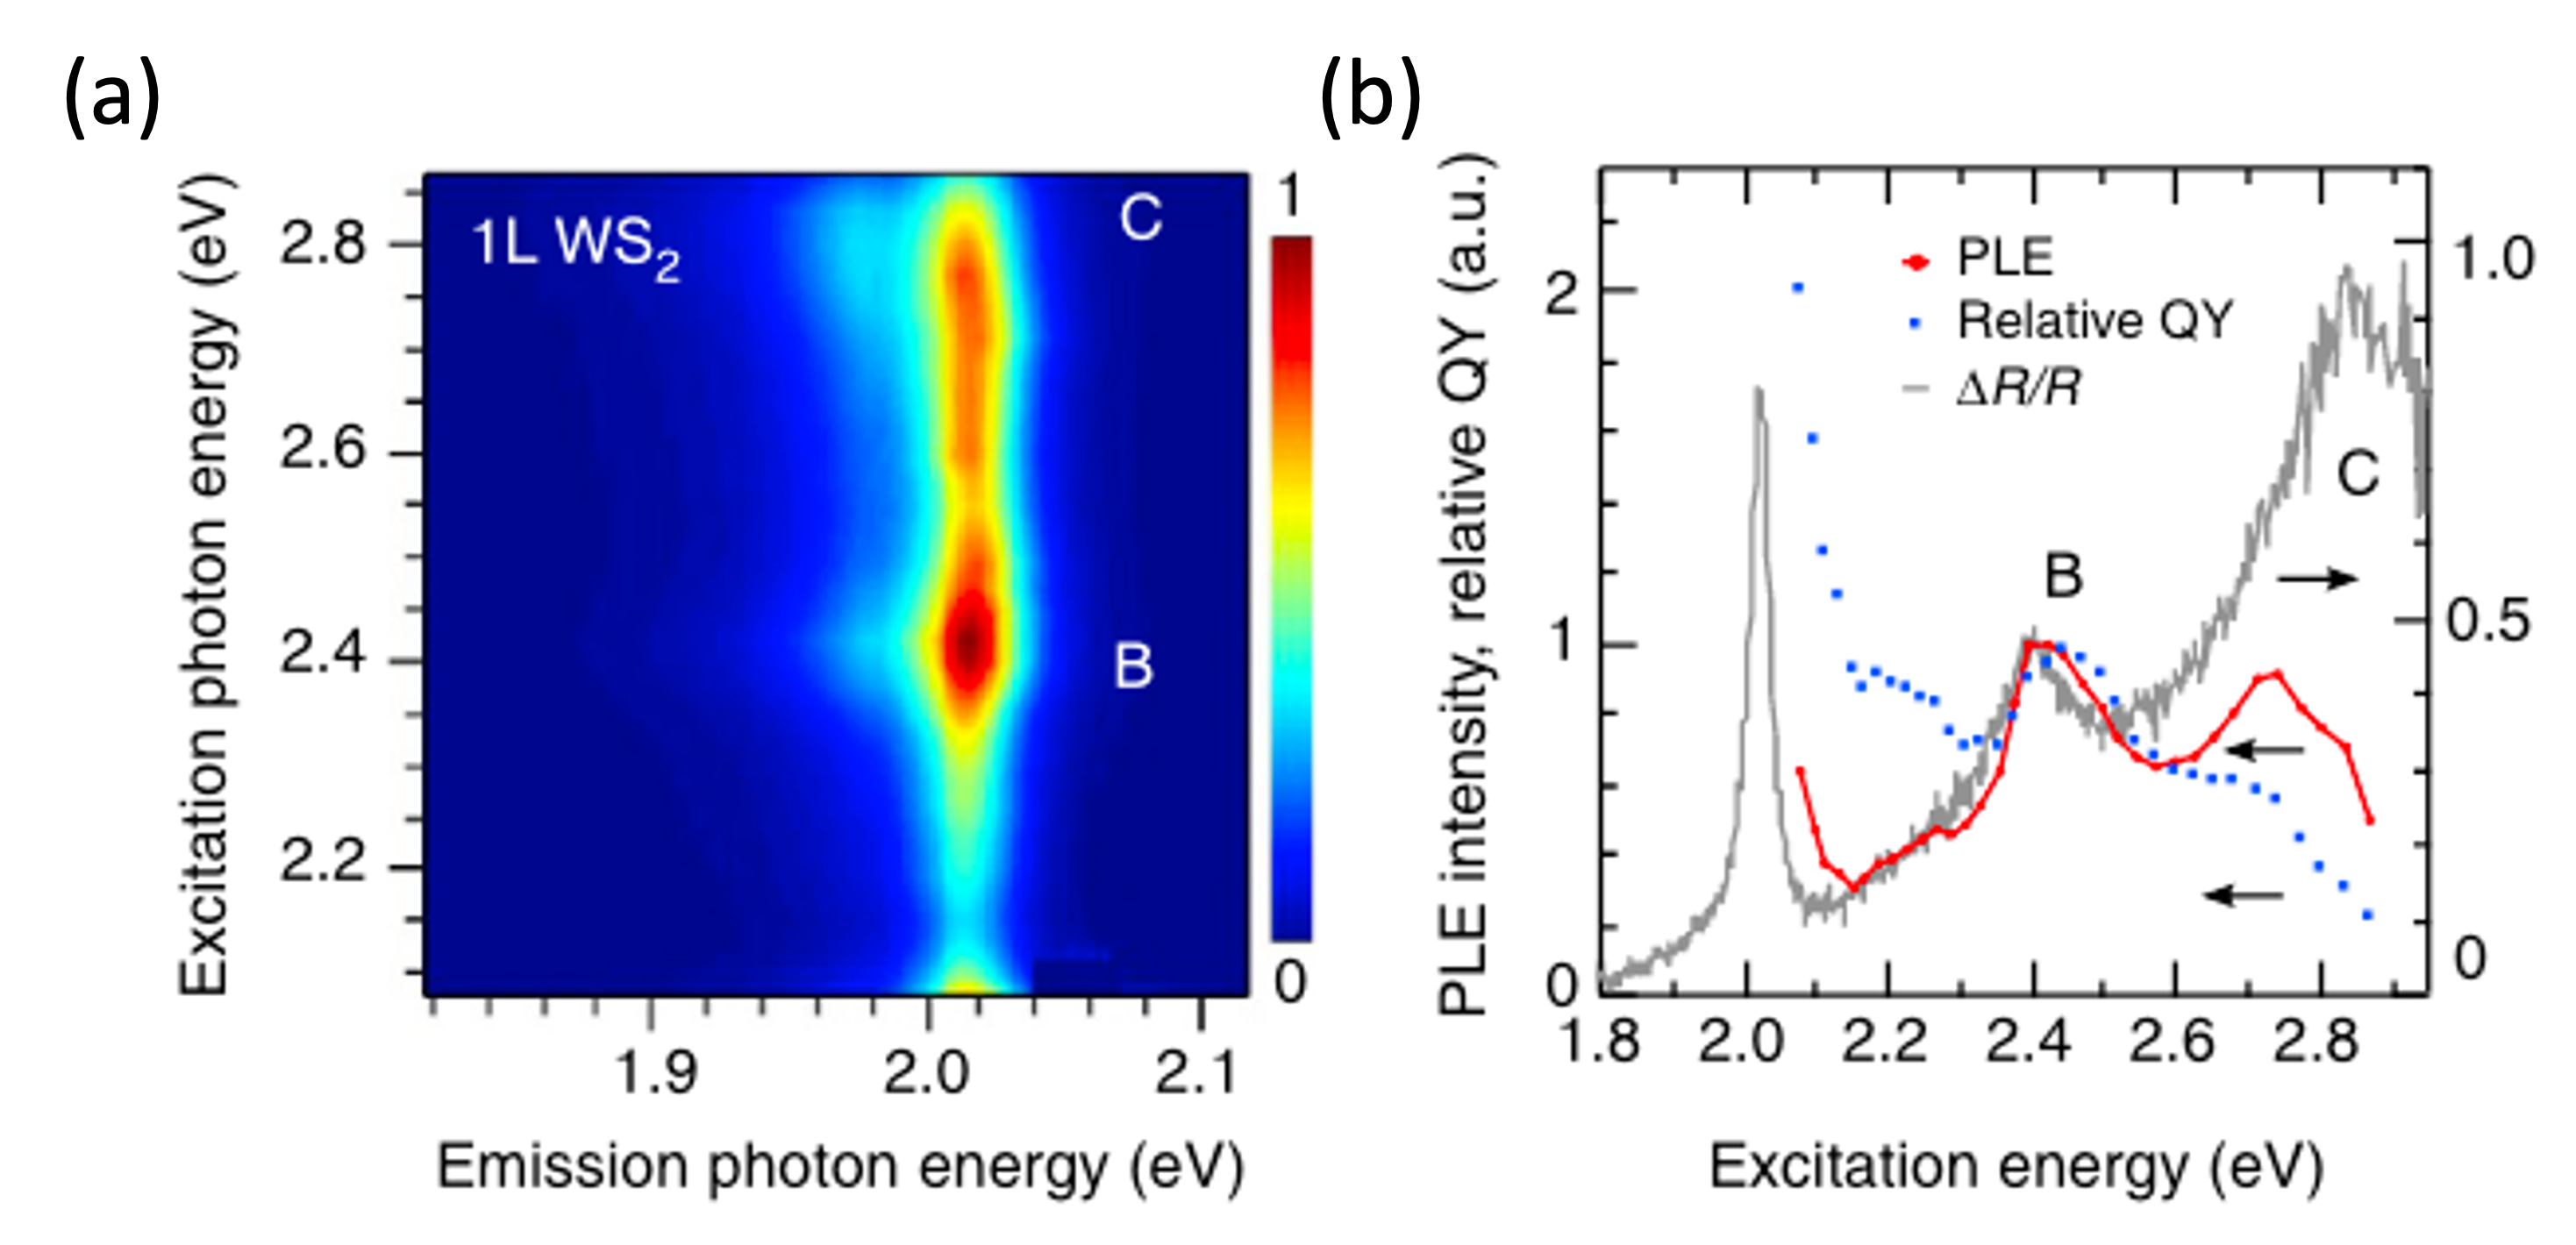
\includegraphics[width=0.9\textwidth]{Figure/Chapter_methodology/PLE_kozawa.png}
    \caption{(a) PLE intensity map of monolayer WS$_2$. (b) PLE spectra and corresponding relative quantum yield (QY) of the band-edge emission in monolayer WS$_2$ \cite{kozawa-2014}.}
    \label{fig:PLE_kozawa}
\end{figure}

As shown in Fig.~\ref{fig:PLE_kozawa}, distinct resonances in the excitation spectrum can lead to markedly different emission intensities, indicating that carriers excited at different energies follow different relaxation pathways. PLE spectroscopy therefore reveals excitation-dependent relaxation processes that are not accessible through PL measurements alone.

In our implementation, the full PL spectrum is recorded as a function of excitation energy at constant excitation power, yielding a three-dimensional dataset (excitation energy, emission energy, intensity). PLE spectra corresponding to specific emission energies are then extracted through post-processing, enabling simultaneous analysis of multiple emission channels.







\subsection{Spatially-resolved Photoluminescence Mapping} % (fold)
\label{sub:chapKeyWord__subsection_3_3}

Thanks to the optical measurement setup shown in Fig.~\ref{fig:optical_setup}, both PL and PLE measurements can be performed at a fixed spatial position. However, such point measurements do not provide information on the spatial distribution of the optical response across the flake.

To access this information, the excitation spot is scanned over the entire region of interest, enabling the reconstruction of spatial maps of the optical properties. This approach provides direct visualization of spatial inhomogeneities, including defects, strain variations, and dielectric disorder.

In particular, the identification of spatially localized defects—one of the central objectives of this work—relies on such mapping, as these features are confined to specific positions and cannot be captured by point measurements.

For this purpose, spatially-resolved photoluminescence mapping is employed, in which the sample is systematically scanned to acquire optical information over the entire flake. In this work, two approaches are used: raster-scanning and hyperspectral mapping.


\vspace{1em}
\noindent \textbf{Raster-scan PL mapping} \\

Spatially-resolved photoluminescence (PL) mapping is performed by scanning the excitation spot across the sample surface in a raster pattern while recording the emitted PL signal at each spatial position. At every point $(x, y)$, a full PL spectrum is acquired under fixed excitation conditions.

An example of a PL intensity map obtained using this method is shown in Fig.~\ref{fig:pl_map}, illustrating the spatial variation of the emission across the flake.

\begin{figure}[htbp]
    \centering
    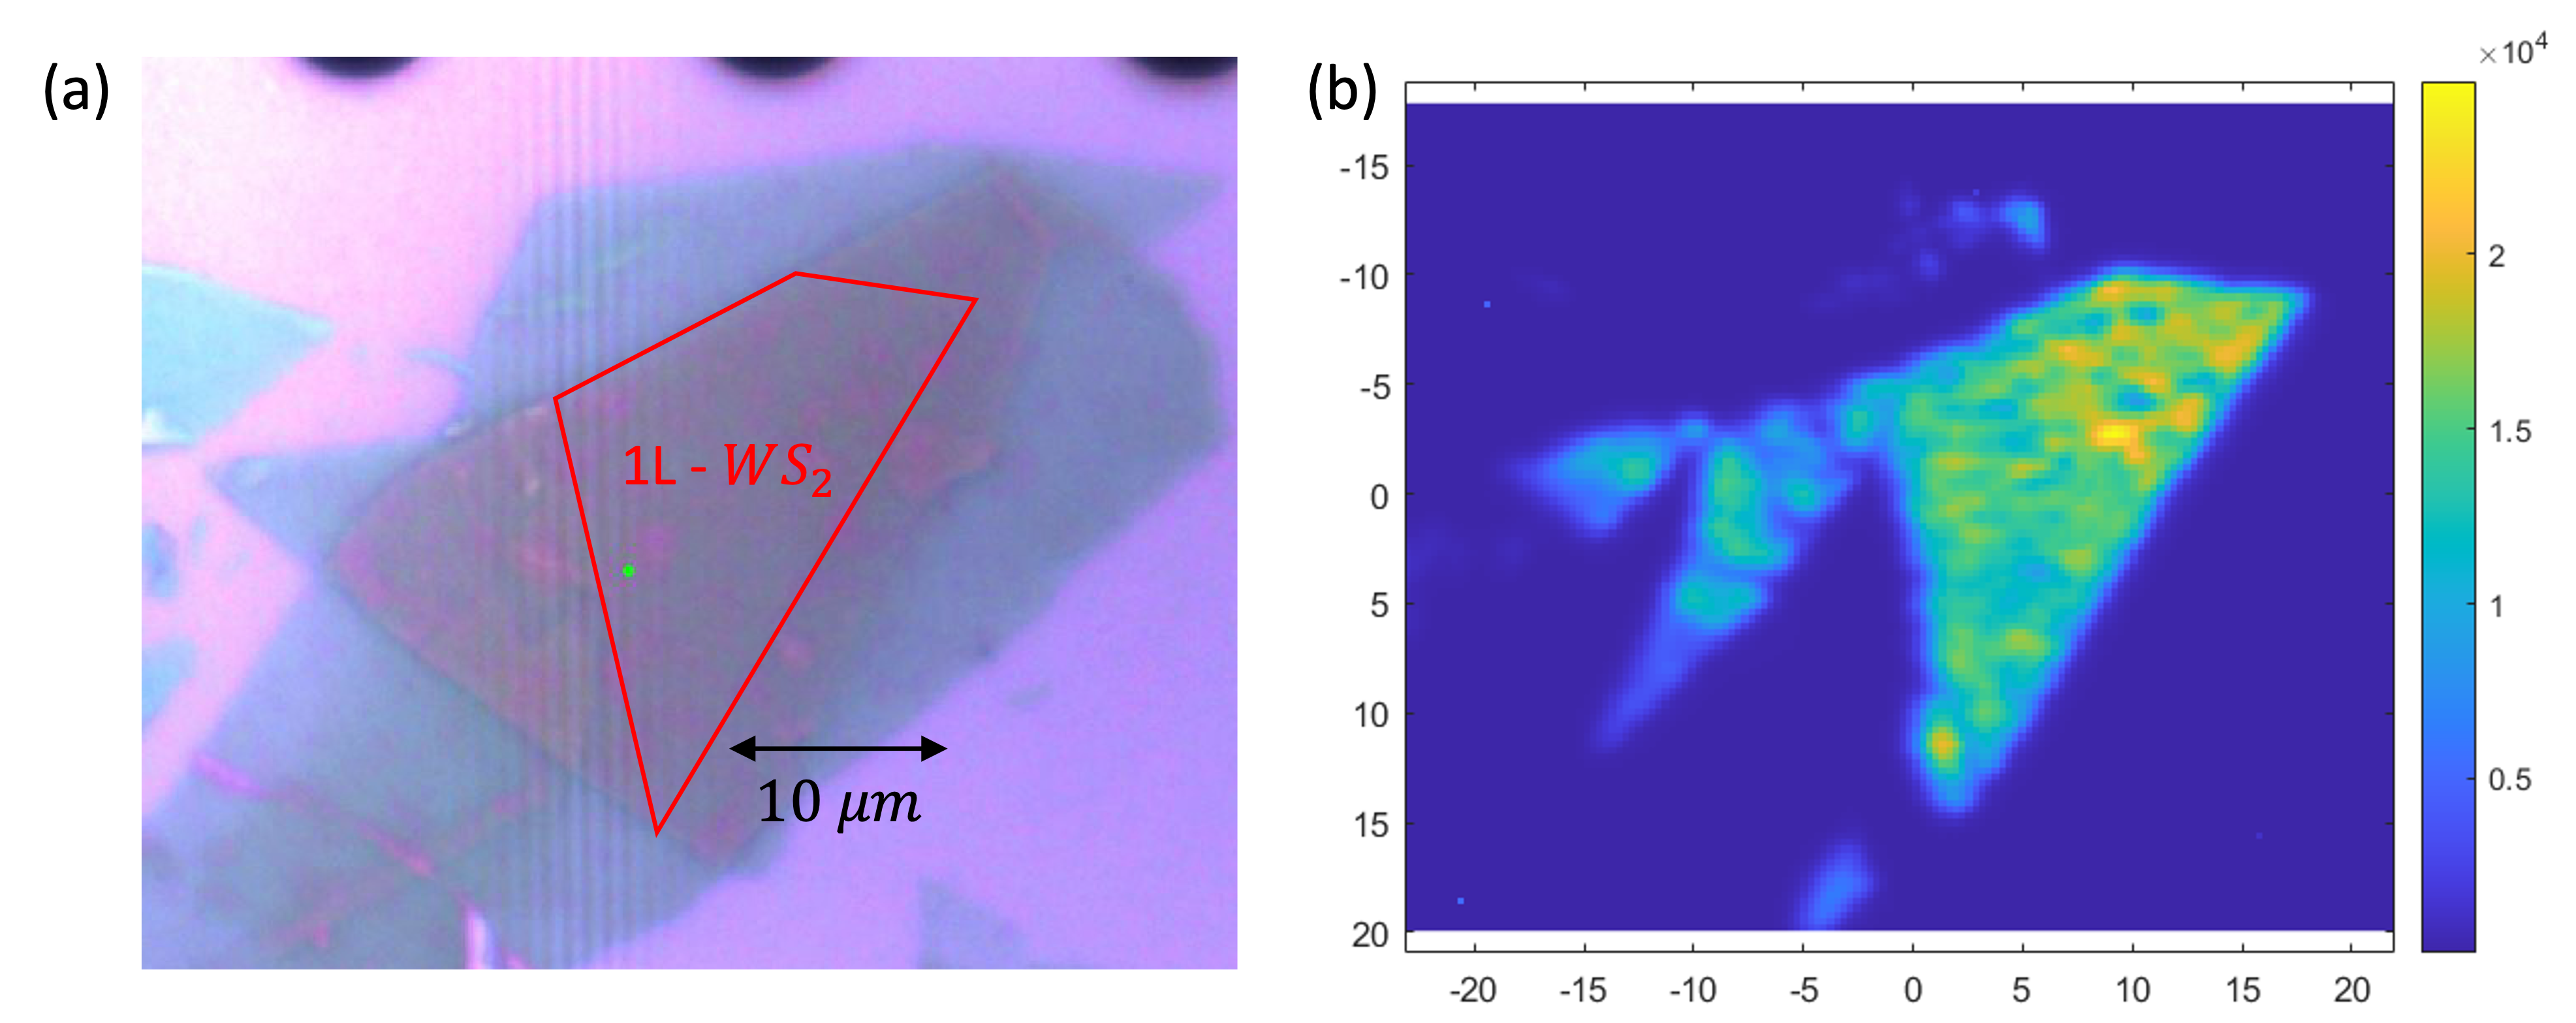
\includegraphics[width=0.9\textwidth]{Figure/Chapter_methodology/pl_map.png}
    \caption{(a) Optical image and (b) corresponding PL intensity map of an hBN-encapsulated WS$_2$ monolayer.}
    \label{fig:pl_map}
\end{figure}

Experimentally, raster scanning is implemented using either a piezoelectric scanner integrated in a cryostat (in-situ) or a commercial optical setup (ex-situ). In the cryogenic configuration, the sample is mounted on a piezoelectric stage that enables precise positioning with respect to the objective. Fine scanning is then performed using a piezoelectric controller to acquire the PL spectrum sequentially at each spatial position, resulting in a spatially-resolved hyperspectral dataset of the emission.


\vspace{1em}
\noindent \textbf{Hyperspectral PL mapping} \\

In contrast to raster-scanning PL mapping, where a full PL spectrum is acquired sequentially at each spatial position, hyperspectral photoluminescence (PL) imaging is based on spectral scanning while preserving the full spatial information at each acquisition step.

In this approach, the entire field of view is projected onto the detector, and a series of PL images is recorded while varying the detection wavelength. Each image corresponds to a two-dimensional intensity distribution at a given wavelength, and the full dataset is reconstructed into a hyperspectral datacube $I(x, y, \lambda)$, from which a complete emission spectrum can be retrieved at every spatial position.

Experimentally, as shown in Fig.~\ref{fig:hyper}, this is implemented by illuminating the full field of view and spectrally filtering the emitted PL using a double spectrometer. By scanning the detection wavelength, wavelength-resolved images are acquired sequentially, forming the hyperspectral dataset.

\begin{figure}[htbp]
    \centering
    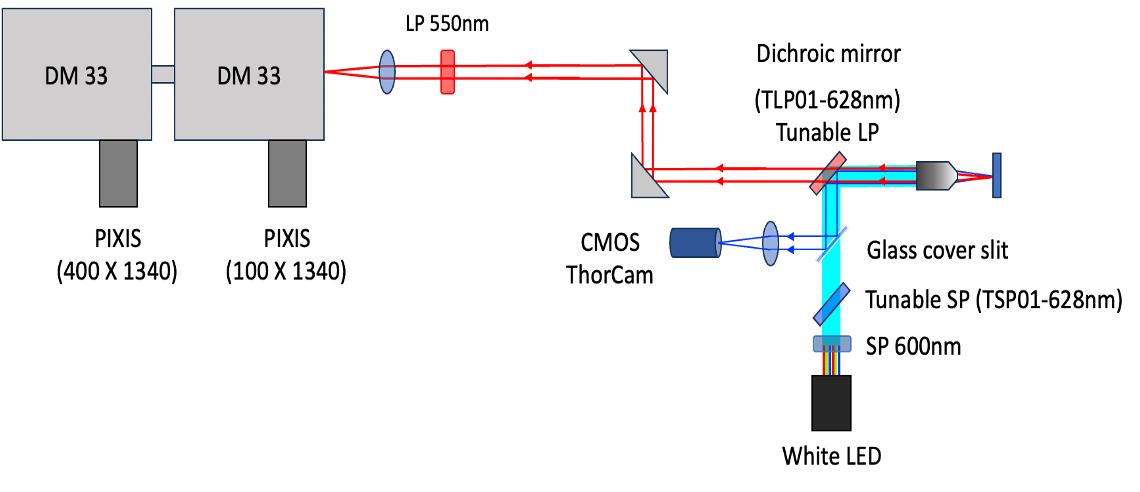
\includegraphics[width=0.9\textwidth]{Figure/Chapter_methodology/hyper.png}
    \caption{Schematic of the hyperspectral photoluminescence (PL) imaging setup.}
    \label{fig:hyper}
\end{figure}

\section{Time-resolved and Quantum Statistical Spectroscopy}
\label{sub:chapKeyWord__subsection_4}

In addition to steady-state optical spectroscopy, time-resolved and quantum statistical measurements are employed to investigate the dynamical and quantum nature of the emission. These techniques provide complementary information on the recombination processes and allow the identification of single-photon emission from localized states.

\subsection{Time-resolved photoluminescence (TRPL) spectroscopy}
\label{sub:chapKeyWord__subsection_4_1}

To access the temporal dynamics of the recombination processes, time-resolved photoluminescence (TRPL) spectroscopy is employed. This technique allows the investigation of the decay dynamics of the emission and provides insight into the nature of the radiative channels.

In this approach, the sample is excited using a pulsed laser source, and the time-dependent PL signal is recorded as a function of the delay after excitation. The emitted photons are spectrally filtered and detected using a time-resolved detection system, allowing the reconstruction of the PL decay dynamics for selected emission features.

By analyzing the temporal evolution of the PL intensity, characteristic lifetimes associated with the emission can be extracted, providing information on the recombination mechanisms and the degree of localization of the excitonic states.

Experimentally, the synchronization signal from the pulsed laser is connected to one channel of a photon counting system, while the emitted photons are detected using single-photon avalanche photodiodes (SPADs) connected to the second channel. This configuration enables time-correlated single-photon counting (TCSPC) measurements of the PL decay.

\subsection{Second-order photon correlation measurements}
\label{sub:chapKeyWord__subsection_4_2}

To investigate the quantum emission characteristics of the sample, single-photon correlation measurements are performed. In particular, the second-order correlation function $g^{(2)}(\tau)$ is measured to determine whether the emission exhibits single-photon behavior.

The second-order correlation function is defined as $g^{(2)}(\tau) = \frac{\langle I(t) I(t+\tau)\rangle}{\langle I(t)\rangle^2}$, representing the normalized intensity correlation between photon detection events separated by a delay $\tau$.

\begin{figure}[htbp]
    \centering
    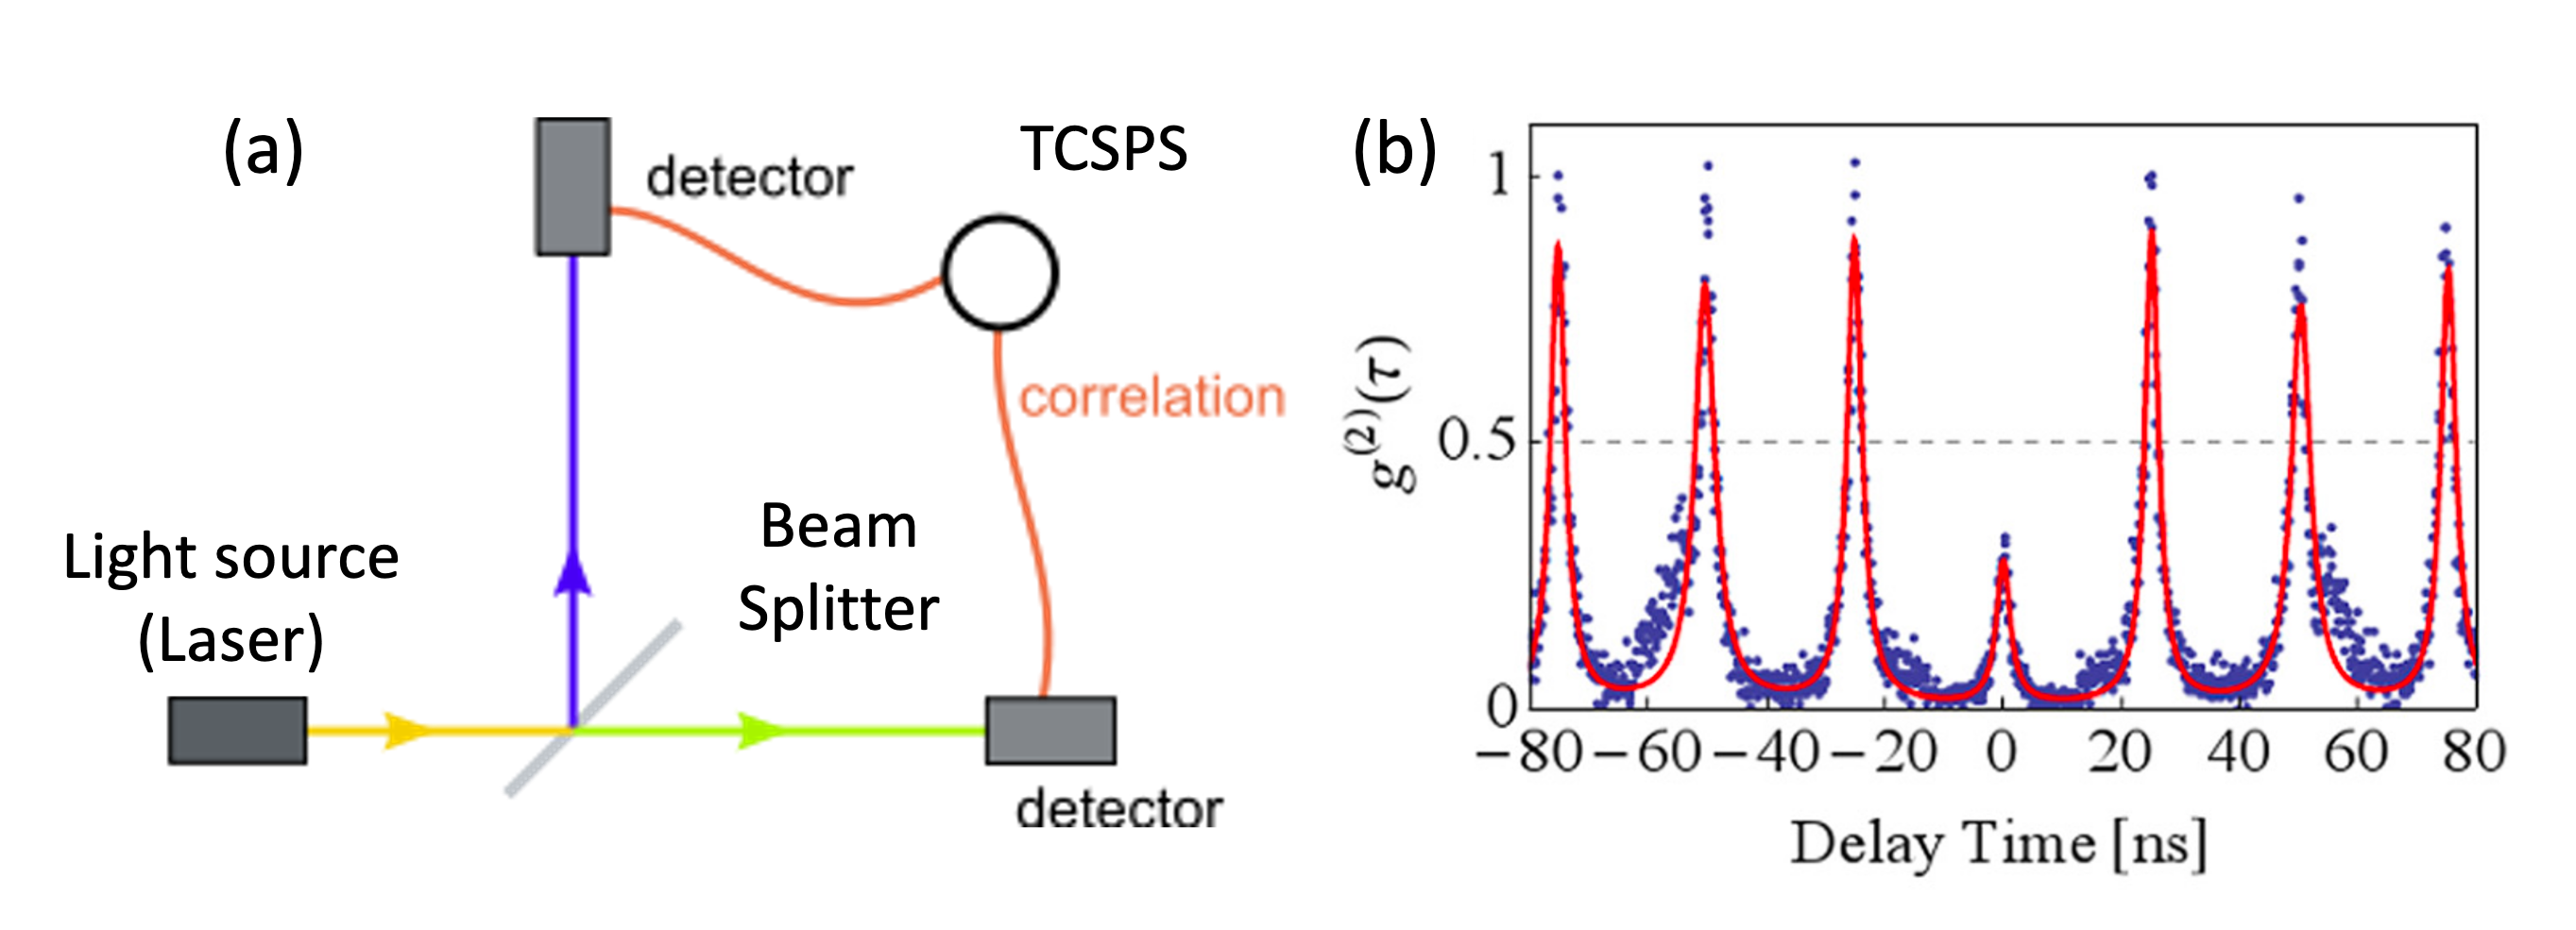
\includegraphics[width=0.9\textwidth]{Figure/Chapter_methodology/g2.png}
    \caption{(a) Schematic of the Hanbury Brown--Twiss interferometer setup. (b) Example of a $g^{(2)}(\tau)$ correlation histogram under pulsed excitation \cite{sandstrom-2014}.}
    \label{fig:g2}
\end{figure}

The measurements are carried out using a Hanbury Brown--Twiss (HBT) interferometer, as shown in Fig.~\ref{fig:g2}. In this configuration, the emitted photons are spectrally filtered using a double spectrometer and then split by a 50:50 beamsplitter. The two output paths are directed to separate single-photon avalanche photodiodes (SPADs), and the detection events are recorded using a photon counting system to evaluate the temporal correlations between the two channels.

The correlation function $g^{(2)}(\tau)$ represents the probability of detecting two photons separated by a delay $\tau$. For an ideal single-photon emitter, $g^{(2)}(0)$ approaches zero, reflecting the absence of simultaneous two-photon events. In practice, a value of $g^{(2)}(0) < 0.5$ is widely accepted as a criterion for confirming single-photon emission. This measurement provides a direct signature of quantum emission statistics beyond classical light behavior.


\section{Conclusion}

In this chapter, the experimental methodology employed throughout this thesis has been presented, including sample fabrication, deterministic transfer, and optical spectroscopy techniques spanning steady-state, spatially-resolved, time-resolved, and quantum statistical measurements. 

Together, these methods establish a comprehensive experimental framework for the investigation of the optical properties of monolayer TMDs and localized excitonic states. The implementation of these techniques enables systematic exploration of the mechanisms governing light emission and will serve as the basis for the results discussed in the following chapters.

% subsection chapKeyWord__subsection_3 (end)


% section chapKeyWord__section_2 (end)

% ---- bibliography
% \printbibheading
\printbibliography[heading=subbibintoc]





\end{document}
